\documentclass[a4paper]{article}
\renewcommand{\epsilon}{\varepsilon}
\newcommand{\triposcourse}{Numerical Analysis}
\usepackage{fancyhdr,titlesec,geometry}
\usepackage[dvipsnames]{xcolor}
\usepackage[many]{tcolorbox}
\usepackage{xifthen}
\usepackage{import}
\usepackage{parskip}
\usepackage{transparent}
\usepackage{mathtools,amssymb,amsfonts,amsthm,bm}   % Math Presets
\usepackage{array,tabularx,booktabs}                % Table Presets
\usepackage{graphicx,wrapfig,float,caption}         % Figure Presets
\usepackage{setspace,multicol}                      % Text Presets
\usepackage{tikz,physics,cancel,tkz-euclide,pgfplots,tikz-3dplot}                    % Physics Presets
\usepackage{amsmath}
\usepackage{mathrsfs}
\usepackage{enumerate}
\usepackage[shortlabels]{enumitem}
\usepackage{hyperref}
\usepackage{lipsum}
\usepackage{IEEEtrantools}
\usepackage{xcomment}
\usepackage{sectsty}
\usepackage{thmtools}
\usepackage{mdframed}
\usepackage{siunitx}
\usepackage{centernot}

\newcommand{\sectionbreak}{\clearpage}

\tdplotsetmaincoords{60}{120}

\usetikzlibrary{arrows.meta}
\usetikzlibrary{decorations.markings}
\usetikzlibrary{decorations.pathmorphing}
\usetikzlibrary{automata, positioning}
\usetikzlibrary{fadings}
\usetikzlibrary{intersections}
\usetikzlibrary{cd}
\usetikzlibrary{patterns}
\usetikzlibrary{shapes.arrows}
\usepgfplotslibrary{colormaps, external}
\pgfarrowsdeclarecombine{twolatex'}{twolatex'}{latex'}{latex'}{latex'}{latex'}
\tikzset{->/.style = {decoration={markings,
                                  mark=at position 1 with {\arrow[scale=1.6]{latex'}}},
                      postaction={decorate}}}
\tikzset{<-/.style = {decoration={markings,
                                  mark=at position 0 with {\arrowreversed[scale=1.6]{latex'}}},
                      postaction={decorate}}}
\tikzset{<->/.style = {decoration={markings,
                                   mark=at position 0 with {\arrowreversed[scale=1.6]{latex'}},
                                   mark=at position 1 with {\arrow[scale=1.6]{latex'}}},
                       postaction={decorate}}}
\tikzset{->-/.style = {decoration={markings,
                                   mark=at position #1 with {\arrow[scale=1.6]{latex'}}},
                       postaction={decorate}}}
\tikzset{-<-/.style = {decoration={markings,
                                   mark=at position #1 with {\arrowreversed[scale=1.6]{latex'}}},
                       postaction={decorate}}}
\tikzset{->>/.style = {decoration={markings,
                                  mark=at position 1 with {\arrow[scale=1.6]{twolatex'}}},
                      postaction={decorate}}}
\tikzset{<<-/.style = {decoration={markings,
                                  mark=at position 0 with {\arrowreversed[scale=1.6]{twolatex'}}},
                      postaction={decorate}}}
\tikzset{<<->>/.style = {decoration={markings,
                                   mark=at position 0 with {\arrowreversed[scale=1.6]{twolatex'}},
                                   mark=at position 1 with {\arrow[scale=1.6]{twolatex'}}},
                       postaction={decorate}}}
\tikzset{->>-/.style = {decoration={markings,
                                   mark=at position #1 with {\arrow[scale=1.6]{twolatex'}}},
                       postaction={decorate}}}
\tikzset{-<<-/.style = {decoration={markings,
                                   mark=at position #1 with {\arrowreversed[scale=1.6]{twolatex'}}},
                       postaction={decorate}}}

\tikzset{
set arrow inside/.code={\pgfqkeys{/tikz/arrow inside}{#1}},
set arrow inside={end/.initial=>, opt/.initial=},
/pgf/decoration/Mark/.style={
    mark/.expanded=at position #1 with
    {
        \noexpand\arrow[\pgfkeysvalueof{/tikz/arrow inside/opt}]{\pgfkeysvalueof{/tikz/arrow inside/end}}
    }
},
arrow inside/.style 2 args={
    set arrow inside={#1},
    postaction={
        decorate,decoration={
            markings,Mark/.list={#2}
        }
    }
},
}

\tikzstyle{circ}=[fill=black, draw=black, shape=circle]
\tikzset{
dot/.style = {circle, fill, minimum size=#1,
              inner sep=0pt, outer sep=0pt},
dot/.default = 5pt% size of the circle diameter 
}
\tikzset{mstate/.style={circle, draw, blue, text=black, minimum width=0.7cm}}
\tikzset{snake it/.style={-stealth,
decoration={snake, 
    amplitude = .4mm,
    segment length = 2mm,
    post length=0.9mm},decorate}}

\def\centerarc[#1](#2)(#3:#4:#5)% Syntax: [draw options](center)(initial angle:final angle:radius)
    { \draw[#1] ($(#2)+({#5*cos(#3)},{#5*sin(#3)})$) arc (#3:#4:#5); }

\hypersetup{
    colorlinks=true,
    linkcolor=blue,
    filecolor=blue,
    citecolor = black,      
    urlcolor=cyan,
    }

%%%%%%%%%%% Snippets %%%%%%%%%%%%%%%%
\newcommand*\widefbox[1]{\fbox{\hspace{2em}#1\hspace{2em}}}
\newcommand{\xint}{\int_{x_1}^{x_2}}
\newcommand{\mw}{\sqrt{m\omega}}
\newcommand{\de}{\delta}
\newcommand{\dde}{\dot{\delta}}
\newcommand{\di}{\delta_i}
\newcommand{\ddi}{\dot{\delta_i}}
\newcommand{\dddi}{\ddot{\delta_i}}
\newcommand{\dipl}{\delta_{i+1}}
\newcommand{\dimi}{\delta_{i-1}}
\newcommand{\ddt}[1]{\frac{{d} #1}{dt}}
\newcommand{\ddtt}[1]{\frac{d^2 #1}{dt^2}}
\newcommand{\ddx}[1]{\frac{d #1}{dx}}
\newcommand{\ddxx}[1]{\frac{d^2 #1}{dx^2}}
\newcommand{\eps}{\epsilon}
\newcommand{\del}[2]{\frac{\partial #1}{\partial #2}}
\newcommand{\deltwo}[2]{\frac{\partial^2 #1}{\partial #2^2}}
\newcommand{\lam}{\lambda}
\newcommand{\Lam}{\Lambda}
\newcommand{\sig}{\sigma}
\newcommand{\Sig}{\Sigma}
\newcommand{\half}{\frac{1}{2}}
\newcommand{\munu}{{\mu\nu}}
\newcommand{\thalf}{\tfrac{1}{2}}
\renewcommand{\div}{\nabla\cdot}
\renewcommand{\curl}{\nabla\times}

\DeclareMathOperator{\orb}{Orb}
\DeclareMathOperator{\stab}{Stab}
\DeclareMathOperator{\adj}{adj}
\DeclareMathOperator{\ccl}{ccl}
\let\var\relax
\DeclareMathOperator{\var}{Var}
\DeclareMathOperator{\cov}{Cov}
\DeclareMathOperator{\corr}{Corr}
\DeclareMathOperator{\Markov}{Markov}
\DeclareMathOperator{\nullity}{nullity}

\newcommand{\bfA}{{\bf A}}
\newcommand{\bfB}{{\bf B}}
\newcommand{\bfC}{{\bf C}}
\newcommand{\bfD}{{\bf D}}
\newcommand{\bfE}{{\bf E}}
\newcommand{\bfF}{{\bf F}}
\newcommand{\bfG}{{\bf G}}
\newcommand{\bfH}{{\bf H}}
\newcommand{\bfI}{{\bf I}}
\newcommand{\bfJ}{{\bf J}}
\newcommand{\bfK}{{\bf K}}
\newcommand{\bfL}{{\bf L}}
\newcommand{\bfM}{{\bf M}}
\newcommand{\bfN}{{\bf N}}
\newcommand{\bfO}{{\bf O}}
\newcommand{\bfP}{{\bf P}}
\newcommand{\bfQ}{{\bf Q}}
\newcommand{\bfR}{{\bf R}}
\newcommand{\bfS}{{\bf S}}
\newcommand{\bfT}{{\bf T}}
\newcommand{\bfU}{{\bf U}}
\newcommand{\bfV}{{\bf V}}
\newcommand{\bfW}{{\bf W}}
\newcommand{\bfX}{{\bf X}}
\newcommand{\bfY}{{\bf Y}}
\newcommand{\bfZ}{{\bf Z}}

\newcommand{\bfa}{{\bf a}}
\newcommand{\bfb}{{\bf b}}
\newcommand{\bfc}{{\bf c}}
\newcommand{\bfd}{{\bf d}}
\newcommand{\bfe}{{\bf e}}
\newcommand{\bff}{{\bf f}}
\newcommand{\bfg}{{\bf g}}
\newcommand{\bfh}{{\bf h}}
\newcommand{\bfi}{{\bf i}}
\newcommand{\bfj}{{\bf j}}
\newcommand{\bfk}{{\bf k}}
\newcommand{\bfl}{{\bf l}}
\newcommand{\bfm}{{\bf m}}
\newcommand{\bfn}{{\bf n}}
\newcommand{\bfo}{{\bf o}}
\newcommand{\bfp}{{\bf p}}
\newcommand{\bfq}{{\bf q}}
\newcommand{\bfr}{{\bf r}}
\newcommand{\bfs}{{\bf s}}
\newcommand{\bft}{{\bf t}}
\newcommand{\bfu}{{\bf u}}
\newcommand{\bfv}{{\bf v}}
\newcommand{\bfw}{{\bf w}}
\newcommand{\bfx}{{\bf x}}
\newcommand{\bfy}{{\bf y}}
\newcommand{\bfz}{{\bf z}}

\newcommand{\mcA}{{\mathcal{A}}}
\newcommand{\mcB}{{\mathcal{B}}}
\newcommand{\mcC}{{\mathcal{C}}}
\newcommand{\mcD}{{\mathcal{D}}}
\newcommand{\mcE}{{\mathcal{E}}}
\newcommand{\mcF}{{\mathcal{F}}}
\newcommand{\mcG}{{\mathcal{G}}}
\newcommand{\mcH}{{\mathcal{H}}}
\newcommand{\mcI}{{\mathcal{I}}}
\newcommand{\mcJ}{{\mathcal{J}}}
\newcommand{\mcK}{{\mathcal{K}}}
\newcommand{\mcL}{{\mathcal{L}}}
\newcommand{\mcM}{{\mathcal{M}}}
\newcommand{\mcN}{{\mathcal{N}}}
\newcommand{\mcO}{{\mathcal{O}}}
\newcommand{\mcP}{{\mathcal{P}}}
\newcommand{\mcQ}{{\mathcal{Q}}}
\newcommand{\mcR}{{\mathcal{R}}}
\newcommand{\mcS}{{\mathcal{S}}}
\newcommand{\mcT}{{\mathcal{T}}}
\newcommand{\mcU}{{\mathcal{U}}}
\newcommand{\mcV}{{\mathcal{V}}}
\newcommand{\mcW}{{\mathcal{W}}}
\newcommand{\mcX}{{\mathcal{X}}}
\newcommand{\mcY}{{\mathcal{Y}}}
\newcommand{\mcZ}{{\mathcal{Z}}}

\newcommand{\bbA}{{\mathbb{A}}}
\newcommand{\bbB}{{\mathbb{B}}}
\newcommand{\bbC}{{\mathbb{C}}}
\newcommand{\bbD}{{\mathbb{D}}}
\newcommand{\bbE}{{\mathbb{E}}}
\newcommand{\bbF}{{\mathbb{F}}}
\newcommand{\bbG}{{\mathbb{G}}}
\newcommand{\bbH}{{\mathbb{H}}}
\newcommand{\bbI}{{\mathbb{I}}}
\newcommand{\bbJ}{{\mathbb{J}}}
\newcommand{\bbK}{{\mathbb{K}}}
\newcommand{\bbL}{{\mathbb{L}}}
\newcommand{\bbM}{{\mathbb{M}}}
\newcommand{\bbN}{{\mathbb{N}}}
\newcommand{\bbO}{{\mathbb{O}}}
\newcommand{\bbP}{{\mathbb{P}}}
\newcommand{\bbQ}{{\mathbb{Q}}}
\newcommand{\bbR}{{\mathbb{R}}}
\newcommand{\bbS}{{\mathbb{S}}}
\newcommand{\bbT}{{\mathbb{T}}}
\newcommand{\bbU}{{\mathbb{U}}}
\newcommand{\bbV}{{\mathbb{V}}}
\newcommand{\bbW}{{\mathbb{W}}}
\newcommand{\bbX}{{\mathbb{X}}}
\newcommand{\bbY}{{\mathbb{Y}}}
\newcommand{\bbZ}{{\mathbb{Z}}}

\newcommand{\mfa}{{\mathfrak{a}}}
\newcommand{\mfb}{{\mathfrak{b}}}
\newcommand{\mfc}{{\mathfrak{c}}}
\newcommand{\mfd}{{\mathfrak{d}}}
\newcommand{\mfe}{{\mathfrak{e}}}
\newcommand{\mff}{{\mathfrak{f}}}
\newcommand{\mfg}{{\mathfrak{g}}}
\newcommand{\mfh}{{\mathfrak{h}}}
\newcommand{\mfi}{{\mathfrak{i}}}
\newcommand{\mfj}{{\mathfrak{j}}}
\newcommand{\mfk}{{\mathfrak{k}}}
\newcommand{\mfl}{{\mathfrak{l}}}
\newcommand{\mfm}{{\mathfrak{m}}}
\newcommand{\mfn}{{\mathfrak{n}}}
\newcommand{\mfo}{{\mathfrak{o}}}
\newcommand{\mfp}{{\mathfrak{p}}}
\newcommand{\mfq}{{\mathfrak{q}}}
\newcommand{\mfr}{{\mathfrak{r}}}
\newcommand{\mfs}{{\mathfrak{s}}}
\newcommand{\mft}{{\mathfrak{t}}}
\newcommand{\mfu}{{\mathfrak{u}}}
\newcommand{\mfv}{{\mathfrak{v}}}
\newcommand{\mfw}{{\mathfrak{w}}}
\newcommand{\mfx}{{\mathfrak{x}}}
\newcommand{\mfy}{{\mathfrak{y}}}
\newcommand{\mfz}{{\mathfrak{z}}}

\newcommand{\mfA}{{\mathfrak{A}}}
\newcommand{\mfB}{{\mathfrak{B}}}
\newcommand{\mfC}{{\mathfrak{C}}}
\newcommand{\mfD}{{\mathfrak{D}}}
\newcommand{\mfE}{{\mathfrak{E}}}
\newcommand{\mfF}{{\mathfrak{F}}}
\newcommand{\mfG}{{\mathfrak{G}}}
\newcommand{\mfH}{{\mathfrak{H}}}
\newcommand{\mfI}{{\mathfrak{I}}}
\newcommand{\mfJ}{{\mathfrak{J}}}
\newcommand{\mfK}{{\mathfrak{K}}}
\newcommand{\mfL}{{\mathfrak{L}}}
\newcommand{\mfM}{{\mathfrak{M}}}
\newcommand{\mfN}{{\mathfrak{N}}}
\newcommand{\mfO}{{\mathfrak{O}}}
\newcommand{\mfP}{{\mathfrak{P}}}
\newcommand{\mfQ}{{\mathfrak{Q}}}
\newcommand{\mfR}{{\mathfrak{R}}}
\newcommand{\mfS}{{\mathfrak{S}}}
\newcommand{\mfT}{{\mathfrak{T}}}
\newcommand{\mfU}{{\mathfrak{U}}}
\newcommand{\mfV}{{\mathfrak{V}}}
\newcommand{\mfW}{{\mathfrak{W}}}
\newcommand{\mfX}{{\mathfrak{X}}}
\newcommand{\mfY}{{\mathfrak{Y}}}
\newcommand{\mfZ}{{\mathfrak{Z}}}

\newcommand{\rma}{\mathrm{a}}
\newcommand{\rmb}{\mathrm{b}}
\newcommand{\rmc}{\mathrm{c}}
\newcommand{\rmd}{\mathrm{d}}
\renewcommand{\dd}{\,\mathrm{d}}
\newcommand{\rme}{\mathrm{e}}
\newcommand{\rmf}{\mathrm{f}}
\newcommand{\rmg}{\mathrm{g}}
\newcommand{\rmh}{\mathrm{h}}
\newcommand{\rmi}{\mathrm{i}}
\newcommand{\rmj}{\mathrm{j}}
\newcommand{\rmk}{\mathrm{k}}
\newcommand{\rml}{\mathrm{l}}
\newcommand{\rmm}{\mathrm{m}}
\newcommand{\rmn}{\mathrm{n}}
\newcommand{\rmo}{\mathrm{o}}
\newcommand{\rmp}{\mathrm{p}}
\newcommand{\rmq}{\mathrm{q}}
\newcommand{\rmr}{\mathrm{r}}
\newcommand{\rms}{\mathrm{s}}
\newcommand{\rmt}{\mathrm{t}}
\newcommand{\rmu}{\mathrm{u}}
\newcommand{\rmv}{\mathrm{v}}
\newcommand{\rmw}{\mathrm{w}}
\newcommand{\rmx}{\mathrm{x}}
\newcommand{\rmy}{\mathrm{y}}
\newcommand{\rmz}{\mathrm{z}}
\newcommand{\rmA}{\mathrm{A}}
\newcommand{\rmB}{\mathrm{B}}
\newcommand{\rmC}{\mathrm{C}}
\newcommand{\rmD}{\mathrm{D}}
\newcommand{\rmE}{\mathrm{E}}
\newcommand{\rmF}{\mathrm{F}}
\newcommand{\rmG}{\mathrm{G}}
\newcommand{\rmH}{\mathrm{H}}
\newcommand{\rmI}{\mathrm{I}}
\newcommand{\rmJ}{\mathrm{J}}
\newcommand{\rmK}{\mathrm{K}}
\newcommand{\rmL}{\mathrm{L}}
\newcommand{\rmM}{\mathrm{M}}
\newcommand{\rmN}{\mathrm{N}}
\newcommand{\rmO}{\mathrm{O}}
\newcommand{\rmP}{\mathrm{P}}
\newcommand{\rmQ}{\mathrm{Q}}
\newcommand{\rmR}{\mathrm{R}}
\newcommand{\rmS}{\mathrm{S}}
\newcommand{\rmT}{\mathrm{T}}
\newcommand{\rmU}{\mathrm{U}}
\newcommand{\rmV}{\mathrm{V}}
\newcommand{\rmW}{\mathrm{W}}
\newcommand{\rmX}{\mathrm{X}}
\newcommand{\rmY}{\mathrm{Y}}
\newcommand{\rmZ}{\mathrm{Z}}

\newcommand{\GL}{\mathrm{GL}}
\newcommand{\Or}{\mathrm{O}}
\newcommand{\PGL}{\mathrm{PGL}}
\newcommand{\PSL}{\mathrm{PSL}}
\newcommand{\PSO}{\mathrm{PSO}}
\newcommand{\PSU}{\mathrm{PSU}}
\newcommand{\SL}{\mathrm{SL}}
\newcommand{\SO}{\mathrm{SO}}
\newcommand{\Spin}{\mathrm{Spin}}
\newcommand{\Sp}{\mathrm{Sp}}
\newcommand{\SU}{\mathrm{SU}}
\newcommand{\Mat}{\mathrm{Mat}}

% Some common notations

\renewcommand{\v}{\mathbf{v}}
\newcommand{\w}{\mathbf{w}}
\renewcommand{\u}{\mathbf{u}}

% Matrix algebras
\newcommand{\gl}{\mathfrak{gl}}
\newcommand{\ort}{\mathfrak{o}}
\newcommand{\so}{\mathfrak{so}}
\newcommand{\su}{\mathfrak{su}}
\newcommand{\uu}{\mathfrak{u}}
\renewcommand{\sl}{\mathfrak{sl}}
\newcommand{\inner}[1]{\left\langle{#1}\right\rangle}
\DeclareMathOperator{\spn}{span}

\newcommand{\mobius}{{M\"{o}bius }}

\renewcommand{\ge}{\geqslant}
\renewcommand{\le}{\leqslant}
\renewcommand{\geq}{\geqslant}
\renewcommand{\leq}{\leqslant}
\renewcommand{\restriction}{\mathord{\upharpoonright}}

\newcommand\independent{\protect\mathpalette{\protect\independenT}{\perp}}
\def\independenT#1#2{\mathrel{\rlap{$#1#2$}\mkern2mu{#1#2}}}

\setlength{\parindent}{0pt}
% \setlength{\parskip}{\baselineskip}
\newcommand{\incfig}[1]{%
    \def\svgwidth{0.4\columnwidth}
    \import{./figures/}{#1.pdf_tex}
}
%%%%%%%%%%%%%%%%%%%%%%%%%%%%%%%%%%%%%

\usepackage[T1]{fontenc}
\usepackage{lmodern,mathrsfs}

%%%%%%%boxed enviroment for final layout%%%%%%%%%%%%%

\newtheoremstyle{mystyle}%
  {}%
  {}%
  {}%
  {}%
  {\sffamily\bfseries}%
  {.}%
  { }%
  {}%

% \renewenvironment{proof}{{\sffamily\bfseries Proof. }}{\qed}

\theoremstyle{mystyle}{
  \newtheorem{theorem}{Theorem}[section]
  \newtheorem{lemma}[theorem]{Lemma}
  \newtheorem{proposition}[theorem]{Proposition}
  \newtheorem{corollary}[theorem]{Corollary}
  \newtheorem{problem}[theorem]{Problem}
  \newtheorem*{claim}{Claim}
  \newtheorem*{slemma}{Lemma}
  \newtheorem*{sprop}{Proposition}
  \newtheorem*{notation}{Notation}

  \newtheorem{inquestion}{Question}
  \newtheorem*{sque}{Question}

  \newtheorem{definition}{Definition}[section]
  \newtheorem{conjecture}{Conjecture}[section]
  \newtheorem{example}{Example}[section]
  \newtheorem*{law}{Law}

  \newtheorem*{remark}{Remark}
  \newtheorem*{note}{Note}
}

\newenvironment{question}[1]
{\renewcommand\theinquestion{#1}\inquestion}
{\endinquestion}

\theoremstyle{definition}{
    \newtheorem*{exercise}{Exercise}}

\tcolorboxenvironment{definition}{
  boxrule=0pt,
  boxsep=2pt,
  colback={White!90!Cerulean},
  enhanced jigsaw, 
  borderline west={2pt}{0pt}{Cerulean},
  sharp corners,
  before skip=10pt,
  after skip=10pt,
  breakable,
  % parbox=false,
}

\tcolorboxenvironment{notation}{
  boxrule=0pt,
  boxsep=2pt,
  colback={White!90!Cerulean},
  enhanced jigsaw, 
  borderline west={2pt}{0pt}{Cerulean},
  sharp corners,
  before skip=10pt,
  after skip=10pt,
  breakable,
  % parbox=false,
}

\tcolorboxenvironment{proposition}{
  boxrule=0pt,
  boxsep=2pt,
  colback={White!90!Yellow},
  enhanced jigsaw, 
  borderline west={2pt}{0pt}{Yellow},
  sharp corners,
  before skip=10pt,
  after skip=10pt,
  breakable,
  % parbox=false,
}

\tcolorboxenvironment{sprop}{
  boxrule=0pt,
  boxsep=2pt,
  colback={White!90!Yellow},
  enhanced jigsaw, 
  borderline west={2pt}{0pt}{Yellow},
  sharp corners,
  before skip=10pt,
  after skip=10pt,
  breakable,
  % parbox=false,
}

\tcolorboxenvironment{theorem}{
  boxrule=0pt,
  boxsep=2pt,
  colback={White!90!Dandelion},
  enhanced jigsaw, 
  borderline west={2pt}{0pt}{Dandelion},
  sharp corners,
  before skip=10pt,
  after skip=10pt,
  breakable,
  % parbox=false,
}

\tcolorboxenvironment{lemma}{
  boxrule=0pt,
  boxsep=2pt,
  blanker,
  borderline west={2pt}{0pt}{Red},
  before skip=10pt,
  after skip=10pt,
  sharp corners,
  left=12pt,
  right=12pt,
  breakable,
  % parbox=false,
}

\tcolorboxenvironment{corollary}{
  boxrule=0pt,
  boxsep=2pt,
  blanker,
  borderline west={2pt}{0pt}{ForestGreen},
  before skip=10pt,
  after skip=10pt,
  sharp corners,
  left=12pt,
  right=12pt,
  breakable,
  % parbox=false,
}

\tcolorboxenvironment{proof}{
  boxrule=0pt,
  boxsep=2pt,
  blanker,
  borderline west={2pt}{0pt}{NavyBlue!80!white},
  before skip=10pt,
  after skip=10pt,
  left=12pt,
  right=12pt,
  breakable,
  % parbox=false,
}

\tcolorboxenvironment{remark}{
  boxrule=0pt,
  boxsep=2pt,
  blanker,
  borderline west={2pt}{0pt}{Green},
  before skip=10pt,
  after skip=10pt,
  left=12pt,
  right=12pt,
  breakable,
  % parbox=false,
}

\tcolorboxenvironment{note}{
  boxrule=0pt,
  boxsep=2pt,
  blanker,
  borderline west={2pt}{0pt}{PineGreen},
  before skip=10pt,
  after skip=10pt,
  left=12pt,
  right=12pt,
  breakable,
  % parbox=false,
}

\tcolorboxenvironment{example}{
  boxrule=0pt,
  boxsep=2pt,
  blanker,
  borderline west={2pt}{0pt}{Black},
  sharp corners,
  before skip=10pt,
  after skip=10pt,
  left=12pt,
  right=12pt,
  breakable,
  % parbox=false,
}

\titleformat*{\section}{\Large\bfseries\sffamily}
\titleformat*{\subsection}{\large\bfseries\sffamily}
\titleformat*{\subsubsection}{\bfseries\sffamily}
\titleformat*{\paragraph}{\bfseries\sffamily}

%%%%%%%%%%%%%%%%%%%%%%%%%%%%%%%%%%%%%%%%%%%%%%%%%%%%

\title{\textbf{\sffamily\triposcourse{} Notes}}
% \usepackage[T1]{fontenc}
\usepackage{crimson}

\theoremstyle{plain}

\theoremstyle{definition}
\newtheorem{theorem}{Theorem}[section]
\newtheorem{lemma}[theorem]{Lemma}
\newtheorem{proposition}[theorem]{Proposition}
\newtheorem{corollary}[theorem]{Corollary}
\newtheorem{problem}[theorem]{Problem}
\newtheorem*{claim}{Claim}
\newtheorem*{slemma}{Lemma}
\newtheorem*{sprop}{Proposition}
\newtheorem*{notation}{Notation}
\newtheorem*{exercise}{Exercise}

\newtheorem{inquestion}{Question}
\newtheorem*{sque}{Question}
\newenvironment{question}[1]
  {\renewcommand\theinquestion{#1}\inquestion}
  {\endinquestion}

\newtheorem{definition}{Definition}[section]
\newtheorem{conjecture}{Conjecture}[section]
\newtheorem{example}{Example}[section]
\newtheorem*{law}{Law}

\theoremstyle{remark}
\newtheorem*{remark}{Remark}
\newtheorem*{note}{Note}

\title{\textbf{\triposcourse{} Notes}}
% \theoremstyle{plain}{
  \newtheorem{theorem}{Theorem}[section]
  \newtheorem{lemma}[theorem]{Lemma}
  \newtheorem{proposition}[theorem]{Proposition}
  \newtheorem{corollary}[theorem]{Corollary}
  \newtheorem*{claim}{Claim}
  \newtheorem*{slemma}{Lemma}
  \newtheorem*{sprop}{Proposition}
  \newtheorem{conjecture}{Conjecture}[section]
  \newtheorem*{law}{Law}
  \newtheorem{inquestion}{Question}
  \newtheorem*{sque}{Question}
}

\theoremstyle{definition}{
  \newtheorem{method}[theorem]{Method}
  \newtheorem{definition}{Definition}[section]
  \newtheorem{example}{Example}[section]
  \newtheorem*{notation}{Notation}
  \newtheorem*{exercise}{Exercise}
}

\theoremstyle{remark}{
  \newtheorem{remark}[theorem]{Remark}
  \newtheorem*{note}{Note}
}

\newenvironment{question}[1]
{\renewcommand\theinquestion{#1}\inquestion}
{\endinquestion}

\title{\textbf{\sffamily\triposcourse{} Notes}}

%layout full
% \geometry{%
%   a4paper,
%   lmargin=2cm,
%   rmargin=2.5cm,
%   tmargin=3.5cm,
%   bmargin=2.5cm,
%   footskip=12pt,
%   headheight=24pt}
% layout trim
% \geometry{
% papersize={379pt, 542pt},
% textwidth=345pt,
% textheight=443pt,
% left=17pt,
% top=54pt,
% right=17pt
% }
% layout a5
\geometry{%
  a5paper,
  lmargin=1cm,
  rmargin=1cm,
  tmargin=2.5cm,
  bmargin=1.5cm,
  footskip=15pt,
  headheight=24pt}
\pagestyle{fancy}
\rhead{{\triposcourse{}}}
\author{jt775}
\AddToHook{cmd/section/before}{\clearpage}

\counterwithin{equation}{section}
\graphicspath{ {./images/} }
\pgfplotsset{compat=1.17}
\begin{document}
\maketitle
\tableofcontents
\clearpage

% \setcounter{section}{-1}
\section{Course description}
\subsection{Polynomial approximation}


\begin{enumerate}
  \item Polynomial interpolation. Lagrange and Newton polynomials. Divided differences.
  \item Error bounds for polynomial interpolation. Chebyshev polynomials. Optimal interpolation knots.

  \item Orthogonal polynomials. Three-term recurrence relation. Least squares polynomial fitting.

  \item Approximation of linear functionals. Numerical integration. Numerical differentiation.

  \item Error of approximation of linear functionals. The Peano kernel theorem. Sharp error bounds.

\end{enumerate}

\subsection{Ordinary differential equations}

\begin{enumerate}
  \setcounter{enumi}{5}
  \item Basics. Euler method. Backward Euler. Trapezoidal rule.
  \item Multistep methods. Order, convergence. Root condition. Dalquist equivalence theorem.

  \item Construction of multistep methods. Adams methods. Backward differentiation formulas (BDF). Relation to numerical quadrature and numerical differentiation formulas.

  \item Runge-Kutta methods. Explicit and implict RK methods. Order of the RK methods.

  \item Stiff ODEs. Linear and A-stability. Stability of multistep methods. Stability of Runge-Kutta methods.

  \item Numerical implementaion. The Milne device. Predictor-corrector scheme. Embedded Runge-Kutta methos.

\end{enumerate}
\subsection{Numerical linear algebra}
\begin{enumerate}
    \setcounter{enumi}{11}
  \item LU factorization. Pivoting.

  \item Existence and uniqueness of the LU factorization. Symmetric positive definite matrices. Diagonally dominant matrices. Sparse and band matrices.

  \item QR factorization. Orthogonal matrices. The Gram-Schmidt orthogonalization.

  \item Givens rotations. Householder reflections.

  \item Linear least squares. Normal equations. QR and least squares.

\end{enumerate}

\subsection{Lecture notes in the class and on the web}
At the beginning of each lecture new handouts will be distributed. Spare handouts of the previous lectures will be available either from myself (after the lecture) or somewhere in the lecture class.

In reasonable circumstances (illness, no spare copies left, etc.), I will send handouts via email.

The lecture notes may appear on the web after the term.

\subsection{Appropriate books}

\begin{enumerate}
    \item (Polynomial approximation)
    
    S. D. Conte, C. de Boor, Elementary numerical analysis: an algorithmic approach, McGrew-Hill 1980
  \item (ODEs)
  
  A. Iserles, A first course in the numerical analysis of differential equations, Cambridge University Press, 2009
  \item (Numerical linear algebra)
  
  No single book known to me.
\end{enumerate}
For all three parts, the lectures and the lecture notes are the best source.

\subsection{What is Numerical Analysis}

Numerical analysis is studying practical algorithms based on solid theoretical background, so in a sense builds a bridge between pure and applied mathematics.

Its main goal is to construct a finite mathematical model that approximates some infinite process with a given accuracy. It is also dealing with the questions of effectiveness, complexity and stability of algorithms that lie in the heart of numerical simulation of reality. Examples include:

\begin{enumerate}
  \item Approximation: reconstruct $f$ from $n$ bits of information;
  \item ODEs, PDEs: $y^{\prime}=f(t, y)$;
  \item Algebraic equations: solve $f(x)=0, f: \mathbb{R}^{n} \rightarrow \mathbb{R}^{m}$, say, linear systems $A \boldsymbol{x}=\boldsymbol{b}$;
  \item Optimization: find $\min _{x \in \Omega} f(x)$;
  \item etc.
\end{enumerate}

\section{Polynomial interpolation}
\subsection{Lagrange and Newton polynomials}
Let $f:[a, b] \rightarrow \mathbb{R}$ be a real-valued continuous function defined on some interval $[a, b]$ and let $(x_{i})_{i=0}^{n}$ be $n+1$ distinct points in $[a, b]$. We wish to construct a polynomial $p$ of degree $n$ which interpolates $f$ at these points, i.e., satisfies
$$
p(x_{i})=f(x_{i}), \quad i=\overline{0, n}, \quad p \in \mathcal{P}_{n} .
$$
\begin{theorem}[Existence and uniqueness]
    Given $f \in C[a, b]$ and $n+1$ distinct points $(x_{i})_{i=0}^{n} \in[a, b]$, there is exactly one polynomial $p \in \mathcal{P}_{n}$ such that $p(x_{i})=f(x_{i})$ for all $i$.
\end{theorem}
\begin{proof}
    (Existence) There is at least one polynomial interpolant $p \in \mathcal{P}_{n}$, the one in the \textbf{Lagrange form},
    \begin{equation}\label{eqn:Lagrange 1}
        p(x)=\sum_{i=0}^{n} f(x_{i}) \ell_{i}(x) \quad \text { with } \quad \ell_{i}(x):=\prod_{\substack{j=0 \\ j \neq i}}^{n} \frac{x-x_{j}}{x_{i}-x_{j}}, \quad i=\overline{0, n},
    \end{equation}
    the $\ell_{i}$ s are called the fundamental Lagrange polynomials. Each $\ell_{i}$ is the product of $n$ linear factors, hence $\ell_{i} \in \mathcal{P}_{n}$. It also equals 1 at $x_{i}$ and vanishes at $x_{j} \neq x_{i}$, i.e., $\ell_{i}(x_{j})=\delta_{i j}$. Therefore $p \in \mathcal{P}_{n}$ and
    $$
    p(x_{j})=\sum_{i=0}^{n} f(x_{i}) \ell_{i}(x_{j})=f(x_{j}) .
    $$
    (Uniqueness) There is at most one polynomial interpolant $p \in \mathcal{P}_{n}$ to $f$ on $(x_{i})_{i=0}^{n}$. For if there are two, $p, q \in \mathcal{P}_{n}$, then the polynomial $r:=p-q$ is of degree $n$ and vanishes at $n+1$ points, whence $r \equiv 0$.
\end{proof}
\begin{remark}
    Let us introduce the so-called \textbf{nodal polynomial}
    $$
    \omega(x):=\prod_{i=0}^{n}(x-x_{i}) .
    $$
    Then, in the expression for $\ell_{i}$, the numerator is simply $\omega(x) /(x-x_{i})$ while the denominator is equal to $\omega^{\prime}(x_{i})$. With that we arrive to a \textbf{compact Lagrange form}
    \begin{equation}\label{eqn:Lagrange 2}
        p(x)=\sum_{i=0}^{n} f(x_{i}) \ell_{i}(x)=\sum_{i=0}^{n} \frac{f(x_{i})}{\omega^{\prime}(x_{i})} \frac{\omega(x)}{x-x_{i}}
    \end{equation}
    The Lagrange forms for the interpolating polynomials are easy to manipulate, but they are unsuitable for numerical evaluation. An alternative is the \textbf{Newton form} which has an \textit{adaptive} nature.
\end{remark}

\begin{method}[The Newton form]
    For $k=\overline{0,n}$, let $p_{k} \in \mathcal{P}_{k}$ be the polynomial interpolant to $f$ on $x_{0}, \ldots, x_{k}$. Then two subsequent $p_{k-1}$ and $p_{k}$ interpolate the same values $f(x_{i})$ for $i \leq k-1$, hence their difference is a polynomial of degree $k$ that vanishes at $k$ points $x_{0}, \ldots, x_{k-1}$. Thus
    \begin{equation}\label{eqn:Newton 1}
        p_{k}(x)-p_{k-1}(x)=A_{k} \prod_{i=0}^{k-1}(x-x_{i}),
    \end{equation}
    with some constant $A_{k}$ which is seen to be equal to the leading coefficient of $p_{k}$. It follows that $p:=p_{n}$ can be built step by step as one constructs the sequence $(p_{0}, p_{1}, \ldots)$, with $p_{k}$ obtained from $p_{k-1}$ by addition the term from the right-hand side of above, so that finally
    $$
    p(x):=p_{n}(x)=p_{0}(x)+\sum_{k=1}^{n}[p_{k}(x)-p_{k-1}(x)]=\sum_{k=0}^{n} A_{k} \prod_{i=0}^{k-1}(x-x_{i})
    $$
\end{method}
\begin{definition}[Divided difference]
    Given $f \in C[a, b]$ and $k+1$ distinct points $(x_{i})_{i=0}^{k} \in[a, b]$, the \textbf{divided difference} $f[x_{0}, \ldots, x_{k}]$ \textbf{of order} $k$ is the leading coefficient of the polynomial $p_{k} \in \mathcal{P}_{k}$ which interpolates $f$ at these points. By definition, it is a symmetric function of the variables $[x_{0}, \ldots, x_{k}]$, and if $f(x)=x^{m}, m \leq k$, then $f[x_{0}, \ldots, x_{k}]=\delta_{k m}$
\end{definition}
With this definition we arrive at the Newton formula for the interpolating polynomial.
\begin{theorem}[Newton formula]
    Given $n+1$ distinct points $(x_{i})_{i=0}^{n}$, let $p_{n} \in \mathcal{P}_{n}$ be the polynomial that interpolates $f$ at these points. Then it may be written in the \textbf{Newton form}
   \begin{align*}
    p_{n}(x)&=f[x_{0}]+f[x_{0}, x_{1}](x-x_{0})+f[x_{0}, x_{1}, x_{2}](x-x_{0})(x-x_{1})+\cdots \\
    &\cdots+f[x_{0}, x_{1}, \ldots, x_{n}](x-x_{0})(x-x_{1}) \cdots(x-x_{n-1}),
   \end{align*}
   or, more compactly,
   \begin{equation}\label{eqn:Divided difference}
    p_{n}(x)=\sum_{k=0}^{n} f[x_{0}, \ldots, x_{k}] \prod_{i=0}^{k-1}(x-x_{i})
   \end{equation}
\end{theorem}
To make this formula of any use, we need an expression for $f[x_{0}, \ldots, x_{k}]$. One such can be derived from the Lagrange formula (\ref{eqn:Lagrange 2}) by identifying the leading coefficient of $p$. This turns to be
\[
    f[x_{0}, \ldots, x_{n}]=\sum_{i=0}^{n} \frac{f(x_{i})}{\omega^{\prime}(x_{i})}, \quad \omega(x):=\prod_{i=0}^{n}(x-x_{i}) .
\]
However, this expression has computational disadvantages as the Lagrange form itself. A useful way to calculate divided difference is again an adaptive (or recurrence) approach.
\begin{theorem}[Recurrence relation]
    For distinct $x_{0}, x_{1}, \ldots, x_{k}$ (with $k \geq 1$), we have
    \begin{equation}\label{eqn:Recurrence relation}
        f[x_{0}, \ldots, x_{k}]=\frac{f[x_{1}, \ldots, x_{k}]-f[x_{0}, \ldots, x_{k-1}]}{x_{k}-x_{0}}
    \end{equation}
\end{theorem}
\begin{proof}
    Let $q_{0}, q_{1} \in \mathcal{P}_{k-1}$ be the polynomials such that 
    \begin{align*}
        & q_0 \text{ interpolates } f \text{ on } (x_0,x_1,\dots,x_{k-1})\\ 
        & q_1 \text{ interpolates } f \text{ on } ~ ~ ~ ~ ~ (x_1,\dots,x_{k-1},x_k)
    \end{align*}
    and consider the polynomial
    \[
        p(x):=\frac{x-x_{0}}{x_{k}-x_{0}} q_{1}(x)+\frac{x_{k}-x}{x_{k}-x_{0}} q_{0}(x), \quad p \in \mathcal{P}_{k}.
    \]
    One readily sees that $p(x_{i})=f(x_{i})$ for all $i$, hence, $p$ is the $k$-th degree interpolating polynomial for $f$. Moreover, the leading coefficient of $p$ is equal to the difference of those of $q_{1}$ and $q_{0}$ divided by $x_{k}-x_{0}$, and that is exactly what the recurrence (\ref{eqn:Recurrence relation}) says.
\end{proof}
\begin{method}
    The recursive formula (\ref{eqn:Recurrence relation}) allows for fast evaluation of the divided difference table
    \begin{center}
        \begin{tikzpicture}
            \matrix(ddtable)[matrix of nodes,
                nodes={anchor=center}
            ]{
                \hline
                $x_i$ & $f[*] = f(*)$ & $f[*,*]$ &[1em] $f[*,*,*]$ &[1em] $f[*,*,*,*]$ \\ \hline
                $x_0$ & $f[x_0]$ &  & &\\ 
                & & $f[x_0,x_1]$ & & \\ 
                $x_1$ & $f[x_1]$ & & $f[x_0,x_1,x_2]$ & \\ 
                & & $f[x_1, x_2]$ & & $f[x_0,x_1,x_2,x_3]$ \\ 
                $x_2$ & $f[x_2]$ & & $f[x_1, x_2, x_3]$ & \\
                & & $f[x_2, x_3]$ & &\\
                $x_3$ & $f[x_3]$ & & & \\ \hline
                & & & & \\
            };
            \draw[-to] (ddtable-2-1) -- (ddtable-2-2);
            \draw[-to] (ddtable-4-1) -- (ddtable-4-2);
            \draw[-to] (ddtable-6-1) -- (ddtable-6-2);
            \draw[-to] (ddtable-8-1) -- (ddtable-8-2);
            \draw[-to] (ddtable-2-2) -- (ddtable-3-3);
            \draw[-to] (ddtable-4-2) -- (ddtable-3-3);
            \draw[-to] (ddtable-4-2) -- (ddtable-5-3);
            \draw[-to] (ddtable-6-2) -- (ddtable-5-3);
            \draw[-to] (ddtable-6-2) -- (ddtable-7-3);
            \draw[-to] (ddtable-8-2) -- (ddtable-7-3);
            \draw[-to] (ddtable-3-3) -- (ddtable-4-4);
            \draw[-to] (ddtable-5-3) -- (ddtable-4-4);
            \draw[-to] (ddtable-5-3) -- (ddtable-6-4);
            \draw[-to] (ddtable-7-3) -- (ddtable-6-4);
            \draw[-to] (ddtable-4-4) -- (ddtable-5-5);
            \draw[-to] (ddtable-6-4) -- (ddtable-5-5);
        \end{tikzpicture}
      \end{center}
    \end{method}
This can be done in $\mathcal{O}(n^{2})$ operations, the outcome is the numbers $\{f[x_{0}, \ldots, x_{k}]\}_{k=0}^{n}$ at the head of the columns which can be used in the Newton form (\ref{eqn:Newton 1}).
\begin{method}[Horner scheme]
    Finally, evaluation of $p$ at a given point $x$ using Newton formula (provided that divided differences $A_{k}:=f[x_{0}, \ldots x_{k}]$ are known) requires just $n$ multiplications, as long as we do it by the \textbf{Horner scheme}
    \begin{align*}
        p_{n}(x)=\{\cdots\{\{A_{n} &\times(x-x_{n-1})+A_{n-1}\} \\ 
        &\times(x-x_{n-2})+A_{n-2}\} \\ 
        &\times(x-x_{n-3})+\cdots+A_{1}\} \times(x-x_{0})+A_{0}.
    \end{align*}
\end{method}
In practice, it may be written as 
\begin{alltt}
S <- f[\(\mathtt{x\sb{0}}\),..., \(\mathtt{x\sb{n}}\)]
for k = n - 1,..., 0
    S <- (\(\mathtt{\hat{x}}\) - \(\mathtt{x\sb{k}}\))S + f[\(\mathtt{x\sb{0}}\),..., \(\mathtt{x\sb{k}}\)]
end\end{alltt}
\subsection{Examples}
The next example derives interpolation polynomials of a function using different methods. 
\begin{example}
    Given the data

\begin{center}
\begin{tabular}{crrrr}
    \toprule
$x_{i}$ & 0 & 1 & 2 & 3 \\
\midrule
$f\left(x_{i}\right)$ & $-3$ & $-3$ & $-1$ & 9 \\\bottomrule
\end{tabular}
\end{center}

find the interpolating polynomial $p \in \mathcal{P}_{3}$ in both Lagrange and Newton forms.
\end{example}
1a) Fundamental Lagrange polynomials
\begin{IEEEeqnarray*}{cCcCrl}
    \ell_{0}(x)&=&\tfrac{(x-1)(x-2)(x-3)}{-6}&=& -&\tfrac{1}{6}\left(x^{3}-6 x^{2}+11 x-6\right), \\
    \ell_{1}(x)&=&\tfrac{x(x-2)(x-3)}{2}&=&&\tfrac{1}{2}\left(x^{3}-5 x^{2}+6 x\right), \\
    \ell_{2}(x)&=&\tfrac{x(x-1)(x-3)}{-2}&=&-&\tfrac{1}{2}\left(x^{3}-4 x^{2}+3 x\right), \\
    \ell_{3}(x)&=&\tfrac{x(x-1)(x-2)}{6}&=&&\tfrac{1}{6}\left(x^{3}-3 x^{2}+2 x\right) .
\end{IEEEeqnarray*}
1b) Lagrange form:
$$
\begin{aligned}
p(x) & =\textstyle(-3) \cdot \ell_{0}(x)+(-3) \cdot \ell_{1}(x)+(-1) \cdot \ell_{2}(x)+9 \cdot \ell_{3}(x) \\
& =\textstyle\left(\frac{1}{2}-\frac{3}{2}+\frac{1}{2}+\frac{3}{2}\right) x^{3}+\left(-3+\frac{15}{2}-2-\frac{9}{2}\right) x^{2}+\left(\frac{11}{2}-9+\frac{3}{2}+3\right) x-3 \\
& =\textstyle x^{3}-2 x^{2}+x-3 .
\end{aligned}
$$
2a) Divided differences:
\begin{center}
\begin{tikzpicture}
    \matrix(dd)[matrix of nodes,
        nodes={anchor=center}
    ]{
        $\widehat{0}$ & $-\overset{*}{3}$ &[.5em]  &[1em] &[1em]\\ 
        & & $\frac{(-3)-(-3)}{1-0} = \overset{*}{0}$ & & \\ 
        $\widehat{1}$ & $-3$ & & $\frac{2-0}{2-0}= \overset{*}{1}$ & \\ 
        & & $\frac{(-1)-(-3)}{2-1}=2$ & & $\frac{4-1}{3-0}=\overset{*}{1}$ \\ 
        $\widehat{2}$ & $-1$ & & $\frac{10-2}{3-1}=4$ & \\
        & & $\frac{9-(-1)}{3-2}=10$ & &\\
        $\widehat{3}$ & $9$ & & & \\
    };
    \draw (dd-1-1.north east) -- (dd-7-1.south east);
    \draw[-to] (dd-1-2) -- (dd-2-3);
    \draw[-to] (dd-3-2) -- (dd-2-3);
    \draw[-to] (dd-3-2) -- (dd-4-3);
    \draw[-to] (dd-5-2) -- (dd-4-3);
    \draw[-to] (dd-5-2) -- (dd-6-3);
    \draw[-to] (dd-7-2) -- (dd-6-3);
    \draw[-to] (dd-2-3) -- (dd-3-4);
    \draw[-to] (dd-4-3) -- (dd-3-4);
    \draw[-to] (dd-4-3) -- (dd-5-4);
    \draw[-to] (dd-6-3) -- (dd-5-4);
    \draw[-to] (dd-3-4) -- (dd-4-5);
    \draw[-to] (dd-5-4) -- (dd-4-5);
\end{tikzpicture}
\end{center}
2b) Newton form:
$$
p(x)=-\overset{*}{3}+\overset{*}{0} \cdot(x-\widehat{0})+\overset{*}{1} \cdot(x-\widehat{0})(x-\widehat{1})+\overset{*}{1} \cdot(x-\widehat{0})(x-\widehat{1})(x-\widehat{2}) .
$$
2c) Horner scheme:
$$
p(x)=\left\{[\overset{*}{1} \cdot(x-\widehat{2})+\overset{*}{1}] \cdot(x-\widehat{1})+\overset{*}{0}\right\} \cdot(x-\widehat{0})-\overset{*}{3}.
$$
\subsection{Some further formulas}
We estimate error terms and give an expression of $ f[x_0, \dots x_k] $. 
\begin{theorem}
    Let $p_{n} \in \mathcal{P}_{n}$ interpolate $f \in C[a, b]$ at $n+1$ distinct points $x_{0}, \ldots, x_{n}$. Then for any $x \notin\left(x_{i}\right)$
    \begin{equation}\label{eqn:error f-p}
        f(x)-p_{n}(x)=f[x_{0}, \ldots, x_{n}, x] \omega(x)
    \end{equation}
\end{theorem}
\begin{proof}
    Given $x_{0}, . ., x_{n}$, let $\bar{x}:=x_{n+1}$ be any other point. Then, by (\ref{eqn:Newton 1}), the corresponding polynomials $p_{n}$ and $p_{n+1}$ are related by
    $$
    p_{n+1}(x)=p_{n}(x)+f\left[x_{0}, \ldots, x_{n}, \bar{x}\right] \omega(x), \quad \omega(x):=\prod_{i=0}^{n}\left(x-x_{i}\right)
    $$
    In particular, putting $x=\bar{x}$, and noticing that $p_{n+1}(\bar{x})=f(\bar{x})$, we obtain
    $$
    f(\bar{x})=p_{n}(\bar{x})+f\left[x_{0}, \ldots, x_{n}, \bar{x}\right] \omega(\bar{x}),
    $$
    the latter equality being the same as (\ref{eqn:error f-p}).
\end{proof}

This theorem shows the error to be ``like the next term'' in the Newton form. However, we cannot evaluate the right-hand side of (\ref{eqn:error f-p}) without knowing the number $f(x)$. But as we now show we can relate it to the $(n+1)$-st derivative of $f$. For this we need a version of the Rolle's theorem:

\begin{lemma}
    If $g \in C^{k}[a, b]$ is zero at $k+\ell$ distinct points, then $g^{(k)}$ has at least $\ell$ distinct zeros in $[a, b]$.
\end{lemma}
\begin{proof}
    By Rolle's theorem, if $\phi \in C^{1}$ is zero at two points, then $\phi^{\prime}$ is zero at an intermediate point. So, we deduce that $g^{\prime}$ vanishes at least at $(k-1)+\ell$ distinct points. Next, applying Rolle to $g^{\prime}$, we conclude that $g^{\prime \prime}$ vanishes at $(k-2)+\ell$ points, and so on.
\end{proof}
\begin{theorem}
    Let $[\bar{a}, \bar{b}]$ be the smallest interval that contains $x_{0}, \ldots, x_{k}$ and let $f \in C^{k}[\bar{a}, \bar{b}]$. Then there exists $\xi \in[\bar{a}, \bar{b}]$ such that
    \begin{equation}\label{eqn:divided difference taylor}
        f[x_{0}, \ldots, x_{k}]=\frac{1}{k !} f^{(k)}(\xi)
    \end{equation}
\end{theorem}
\begin{proof}
    Let $p \in \mathcal{P}_{k}$ be the interpolating polynomial to $f$ on $\left(x_{i}\right)$. The error function $f-p$ has at least $k+1$ zeros in $[\bar{a}, \bar{b}]$ so, by Rolle's theorem, $f^{(k)}-p^{(k)}$ must vanish at some $\xi \in[\bar{a}, \bar{b}]$, i.e.,
    $$
    p^{(k)}(\xi)=f^{(k)}(\xi)
    $$
    On the other hand, if $p(x)=a_{k} x^{k}+$ (lower order terms), then (for any $\xi$)
    $$
    p^{(k)}(\xi)=k ! a_{n}=: k ! f[x_{0}, \ldots, x_{n}] .
    $$
\end{proof}

\section{Error bounds for polynomial interpolation}
Here we study the \textbf{interpolation error}
\[
    e_n(x) = f(x) - p_n(x),\quad p_n\in \mathcal{P}_n,
\]
for the class of differentiable functions $f$ that possess $n+1$ continuous derivatives on the interval $[a,b]$; we denote this class by $C^{n+1}[a,b]$. 
\begin{theorem}
    Let $f \in C^{n+1}[a, b]$, and let $p_n \in \mathcal{P}_n$ interpolate $f$ at $n+1$ points $\left(x_i\right)_{i=0}^n \in[a, b]$, and let $\omega(x):=\prod_{i=0}^n\left(x-x_i\right)$. Then for every $x \in[a, b]$ there exists $\xi \in[a, b]$ such that
    \begin{equation}\label{eqn:error bound}
        f(x)-p_n(x)=\frac{1}{(n+1) !} \omega(x) f^{(n+1)}(\xi)
    \end{equation}
\end{theorem} 
\begin{proof}
    If $x$ coincides with any $x_i$ from the interpolating set, then both sides vanish, hence the formula trivially holds. So, we let $x$ be any other fixed point, and consider the function
    \[
    \phi(t):=[f(t)-p(t)]-c_x \omega(t),
    \]
    with \textit{some} constant $c_x$. For \textit{any} $c_x, \phi(t)=0$ at $n+1$ points $t=x_2$, and we choose \textit{particular} $c_x$ so that $\phi(t)=0$ at $t=x$ as well, i.e.,
    \[
    c_x:=\frac{f(x)-p(x)}{\omega(x)} .
    \]
    Then $\phi$ has $n+2$ distinct zeros hence, by Rolle's theorem, $\phi^{(n+1)}(\xi)=0$ for some $\xi \in[a, b]$. So,
    \[
    0=\phi^{(n+1)}(\xi)=\left[f^{(n+1)}(\xi)-p^{(n+1)}(\xi)\right]-c_x \omega^{(n+1)}(\xi)=f^{(n+1)}(\xi)-c_x(n+1) !
    \]
    whence
    \[
    c_x:=\frac{f(x)-p(x)}{\omega(x)}=\frac{1}{(n+1) !} f^{(n+1)}(\xi),
    \]
    and that is the same as RHS.
\end{proof}

The equality (\ref{eqn:error bound}) with the value $f^{(n+1)}(\xi)$ for some $\xi$ is of hardly any use. Usually one has a bound for $f^{(n+1)}$ in terms of some norm, e.g., the $L_{\infty}$-norm (the max-norm)
\[
\|g\|_{\infty}:=\|g\|_{L_{\infty}[a, b]}:=\max _{t \in[a, b]}|g(t)| .
\]
Then estimate (\ref{eqn:error bound}) takes the form
\begin{equation}\label{eqn:2.2}
    \left|f(x)-p_n(x)\right| \leq \frac{1}{(n+1) !}|\omega(x)|\left\|f^{(n+1)}\right\|_{\infty}
\end{equation}
If we want to find the maximal error over the interval, then maximizing first the right- and then the left-hand side over $x \in[a, b]$ we get yet one more error bound for polynomial interpolation
\begin{equation}\label{eqn:2.3}
    \left\|f-p_{\Delta}\right\|_{\infty} \leq \frac{1}{(n+1) !}\left\|\omega_{\Delta}\right\|_{\infty}\left\|f^{(n+1)}\right\|_{\infty}
\end{equation}
Here we put the lower index in $\omega_{\Delta}$ in order to emphasize dependence of $\omega(x):=\prod_{i=0}^n\left(x-x_i\right)$ on the sequence of interpolating points $\Delta:=\left(x_i\right)_{i=0}^n$. The choice of $\Delta$ makes a big difference!

\begin{example}
    Consider interpolation of the function $\displaystyle f(x) = \frac{1}{1+x^2},\ x\in [-5,5]$. 
    \begin{center}
        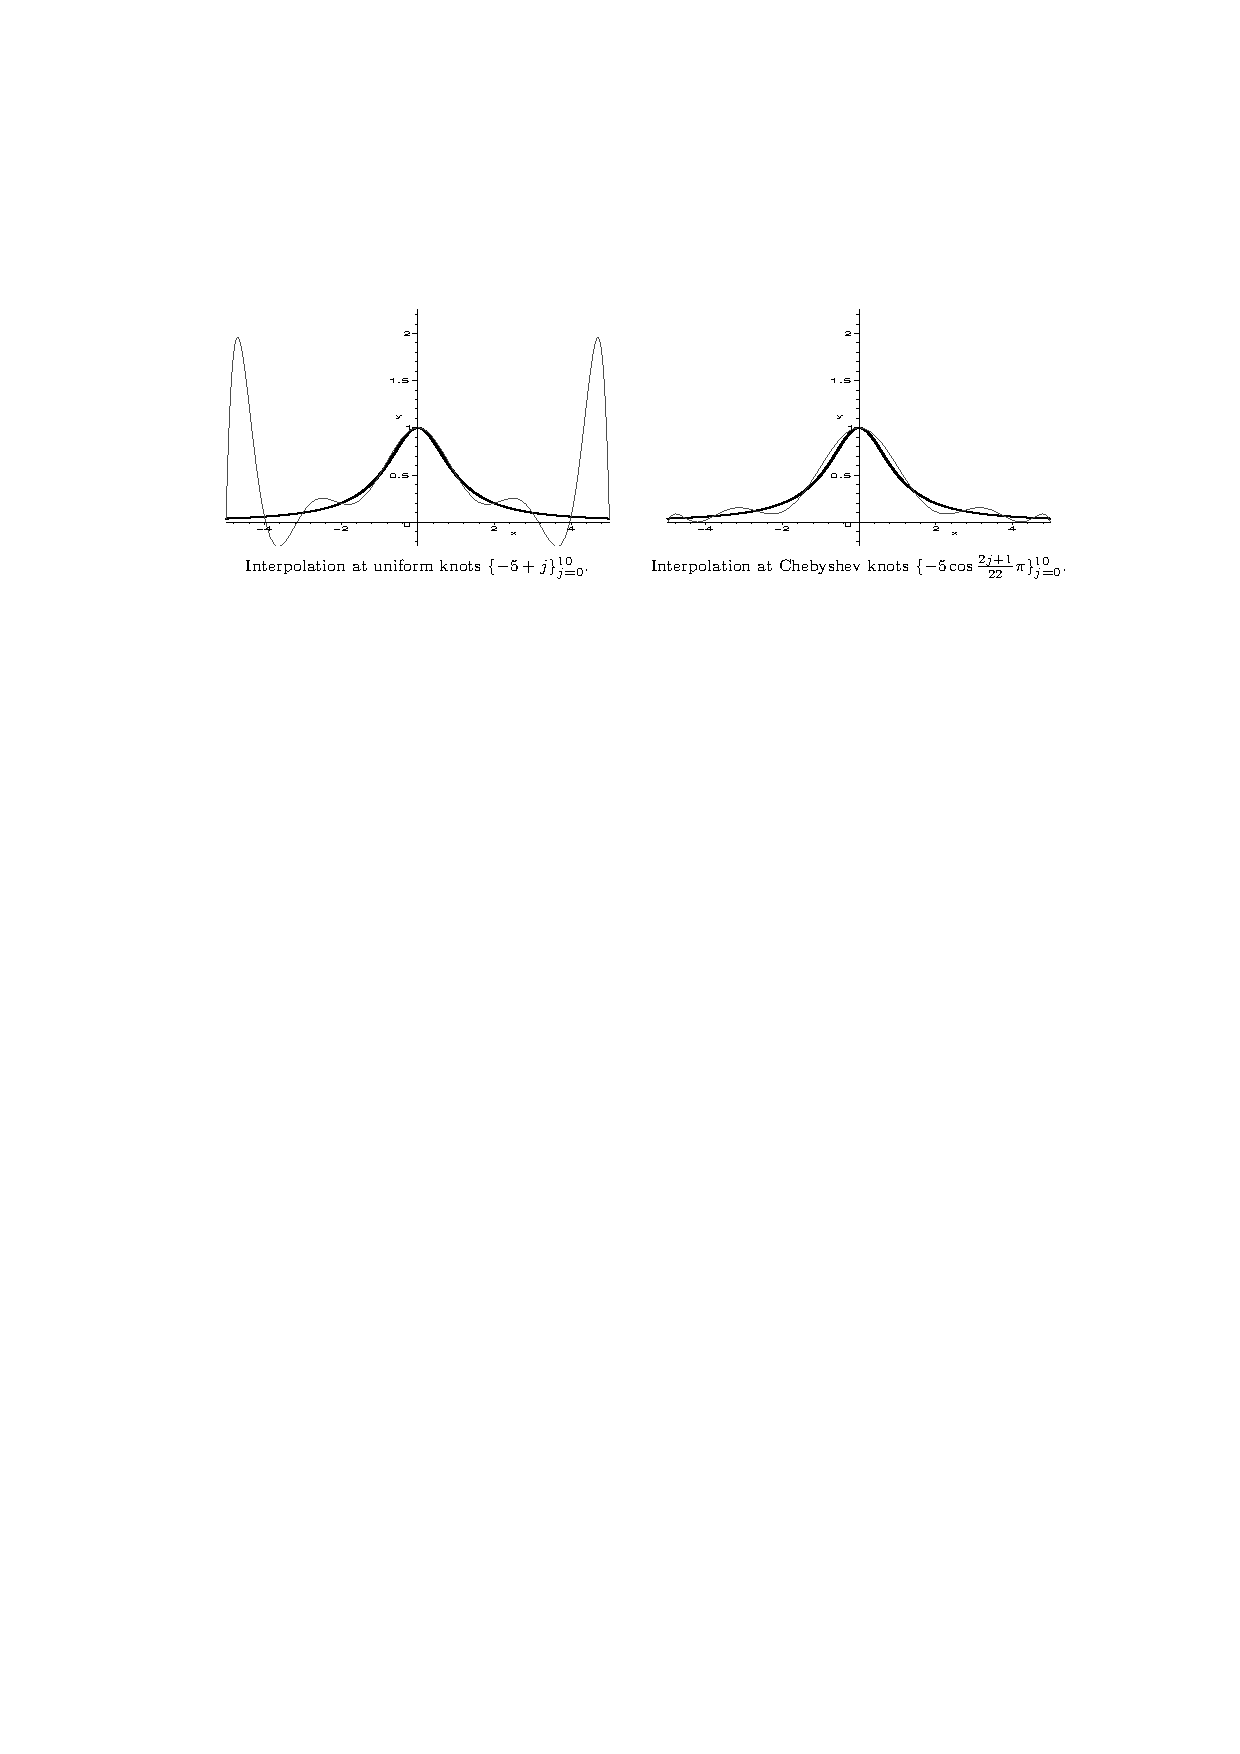
\includegraphics[scale=.85]{NA1}
    \end{center}
\end{example}

\begin{definition}
    The Chebyshev polynomial of degree $n$ on $[-1,1]$ is defined by
    \[
    T_n(x)=\cos n \theta, \quad x=\cos \theta, \quad \theta \in[0, \pi] .
    \]
    (Or just $T_n(x)=\cos (n \arccos x)$, with $x \in[-1,1]$.)
\end{definition}

One sees at once that, on $[-1,1]$,
\begin{enumerate}
    \item  $T_n$ takes its maximal absolute value 1 with alternating signs $n+1$ times:
    \[
    \left\|T_n\right\|_{\infty}=1, \quad T_n\left(t_k\right)=(-1)^k, \quad t_k=\cos \tfrac{\pi k}{n}, \quad k=\overline{0, n}
    \]
    \item $T_n$ has $n$ distinct zeros: $\quad T_n\left(x_k^*\right)=0, \quad x_k^*=\cos \frac{2 k-1}{2 n} \pi, \quad k=\overline{1, n}$.
\end{enumerate}

\begin{lemma}
    The Chebyshev polynomials $T_n$ satisfy the recurrence relation
    \begin{align}
        & T_0(x) \equiv 1, \quad T_1(x)=x, \label{eqn:2.4}\\
        & T_{n+1}(x)=2 x T_n(x)-T_{n-1}(x), \quad n \geq 1 .\label{eqn:2.5}
    \end{align}
    In particular, $T_n$ is an algebraic polynomial of degree $n$ with the leading coefficient $2^{n-1}$.
\end{lemma}
\begin{proof}
    Expressions (\ref{eqn:2.4}) are straightforward, the recurrence follows via the substitution $x=\cos \theta$ into identity $\cos (n+1) \theta+\cos (n-1) \theta=2 \cos \theta \cos n \theta$.
\end{proof}

\begin{theorem}
    On the interoal $[-1,1]$, among all polynomials of degree $n$ with the leading coefficient equal to one, the Chebyshev polynomial $\gamma T_n$ has the smallest max-norm, i.e.,
    \[
    \inf _{\left(a_i\right)}\left\|x^n+a_{n-1} x^{n-1}+\cdots+a_0\right\|_{\infty}=\left\|\gamma T_n\right\|_{\infty}=\gamma, \quad \gamma:=1 / 2^{n-1} .
    \]
\end{theorem}
\begin{proof}
    Suppose there is a polynomial $q_n(x)=x^n+a_{n-1} x^{n-1}+\cdots+a_0$ such that $\|q\|_{\infty}<\gamma$, and set
    \[
    r:=\gamma T_n-q_n .
    \]
    The leading coefficients of both $q_n$ and $\gamma T_n$ are equal 1 , thus $r$ is of degree at most $n-1$.

    Further, at $n+1$ points $t_k:=\cos \frac{\pi k}{n}$, the Chebyshev polynomial $\gamma T_n$ takes the values $\pm \gamma$ alternatively, while by assumption $\left|q_n\left(t_k\right)\right|<\gamma$, hence $r=\gamma T_n-q_n$ alternates in sign at these $n+1$ points, therefore it has a zero in each of $n$ intervals $\left(t_k, t_{k+1}\right)$, i.e. at least $n$ zeros in the interval $[-1,1]$, a contradiction to $r \in \mathcal{P}_{n-1}$.
\end{proof}

\begin{corollary}
    For $\Delta=\left(x_i\right)_{i=0}^n \subset[-1,1]$, let $\omega_{\Delta}(x)=\prod_{i=0}^n\left(x-x_i\right)$. Then, for all $n$, we have
    \[
    \inf _{\Delta}\left\|\omega_{\Delta}\right\|_{\infty}=\left\|\omega_{{\Delta}_{*}}\right\|_{\infty}=1 / 2^n .
    \]
\end{corollary}

\begin{theorem}
    For $f \in C^{n+1}[-1,1]$, the best choice of interpolating points is $\Delta_*=\left(x_i^*\right)=\left(\cos \frac{2 i+1}{2 n+2} \pi\right)_{i=0}^n$ and
    \[
    \left\|f-p_{\Delta_*}\right\|_{\infty} \leq \frac{1}{2^n} \frac{1}{(n+1) !}\left\|f^{(n+1)}\right\|_{\infty}
    \]
\end{theorem}

\begin{example}
    For $f(x)=e^x$, and $x \in[-1,1]$, the error of approximation provided by interpolating polynomial of degree 9 with 10 Chebyshev knots is bounded by
    \[
    \left|e^x-p_9(x)\right| \leq \frac{1}{2^9} \frac{1}{10 !} e \leq 1.5 \cdot 10^{-9}
    \]
\end{example}

\section{Orthogonal polynomials}
\subsection{The three-term recurrence relation}
Consider $\mathbb{X}=C[a, b]$, the space of all continuous real-valued functions $f:[a, b] \rightarrow \mathbb{R}$, and define a \textbf{scalar} (or \textbf{inner}) \textbf{product} on $C[a, b]$ by
\begin{equation}\label{eqn:3.1}
    (f, g):=(f, g)_w:=\int_a^b f(x) g(x) w(x) d x .
\end{equation}
Here $w$, the so-called \textbf{weight function}, is a fixed positive function, such that the integral $\int h(x) w(x) d x$ exists for all $h \in C[a, b]$.

We denote by $\mathcal{P}_n$ the space of all algebraic polynomials of degree (at most) $n$, i.e., $p \in \mathcal{P}_n$ if $p(x)=\sum_{k=0}^n a_k x^k$. If the leading coefficent $a_n$ equals 1 , then $p$ is called a \textbf{monic} polynomial. Given a scalar product (\ref{eqn:3.1}), we say that $Q_n \in \mathcal{P}_n$ is the $n$\textbf{-th} \textbf{orthogonal polynomial} if
\[
\left(Q_n, p\right)=0 \quad \forall p \in \mathcal{P}_{n-1} .
\]
Different weights lead to different orthogonal polynomials.

\begin{lemma}
    For every $n \in \mathbb{N}$, there exists a unique monic orthogonal polynomial $Q_n \in \mathcal{P}_n$. Any $p \in \mathcal{P}_n$ is uniquely expressible as a linear combination
    \begin{equation}\label{eqn:3.2}
        p=\sum_{k=0}^n c_k Q_k, \quad c_k=\left(p, Q_k\right) /\left\|Q_k\right\|^2
    \end{equation}
\end{lemma}
\begin{proof}
    We apply the Gram-Schmidt orthogonalization algorithm for the linearly independent sequence of monomials $\left(1, x, \ldots, x^n, \ldots\right)$. Starting with $Q_0 \equiv 1$ we set
\[
Q_n(x):=x^n-\sum_{k=0}^{n-1} \frac{\left(x^n, Q_k\right)}{\left(Q_k, Q_k\right)} Q_k(x), \quad n=1,2, \ldots
\]
Then, from construction, $\left(Q_n, Q_k\right)=0$, i.e., $Q_n$ is orthogonal to each previous $Q_k$. Also, we have $x^n \in \operatorname{span}\left(Q_k\right)_{k=0}^n$, hence $\mathcal{P}_n=\operatorname{span}\left(Q_k\right)_{k=0}^n$. Therefore $Q_n \perp \mathcal{P}_{n-1}$, and any $p \in \mathcal{P}_n$ has an expansion (\ref{eqn:3.2}). Each coefficient $c_k$ in (\ref{eqn:3.2}) is uniquely determined by multiplying both sides (in the scalar product sense) with $Q_k$.

If $\widetilde{Q}_n$ is another $n$-th monic orthogonal polynomial, then $p:=Q_n-\widetilde{Q}_n$ belongs to $\mathcal{P}_{n-1}$, therefore $(p, p)=\left(Q_n-\widetilde{Q}_n, p\right)=0$. Hence $p \equiv 0$ (by the scalar product property), i.e., $\widetilde{Q}_n \equiv Q_n$.
\end{proof}
\begin{remark}
    For practical construction of orthogonal polynomials the Gram-Schmidt is not of much help, for it leads to loss of accuracy due to imprecisions in calculation of scalar products. A considerably better procedure is being provided by the next theorem.
\end{remark}

\begin{theorem}[The three-term recurrence relation]
    Monic orthogonal polynomials satisfy the relation
    \begin{equation}\label{eqn:3.3}
        Q_{n+1}(x)=\left(x-a_n\right) Q_n(x)-b_n Q_{n-1}(x), \quad n=0,1, \ldots
    \end{equation}
    where $Q_{-1}(x) \equiv 0, Q_0(x) \equiv 1$, and
    \begin{equation}\label{eqn:3.4}
        a_n=\frac{\left(x Q_n, Q_n\right)}{\left(Q_n, Q_n\right)}, \quad b_n=\frac{\left(Q_n, Q_n\right)}{\left(Q_{n-1}, Q_{n-1}\right)}>0
    \end{equation}
\end{theorem}
\begin{proof}
    Based on (\ref{eqn:3.2}), let us look at the coefficients of the expansion
    \[
    x Q_n(x)=\sum_{k=0}^{n+1} c_k Q_k(x), \quad c_k=\frac{\left(x Q_n, Q_k\right)}{\left(Q_k, Q_k\right)}=\frac{\left(Q_n, x Q_k\right)}{\left(Q_k, Q_k\right)},
    \]
    using the last (equivalent) formula for $c_k$.

    $k=n+1 \to  c_{n+1}=1$, since both $x Q_n(x)$ and $Q_{n+1}(x)$ are monic polynomials of degree $n+1$.

    $k=n \to  c_n=a_n$ in (\ref{eqn:3.4}).

    $k=n-1 \to $ Because of monicity, we have the equality $x Q_{n-1}=Q_n+p_{n-1}$ where $p_{n-1} \in \mathcal{P}_{n-1}$, so that $\left(Q_n, x Q_{n-1}\right)=\left(Q_n, Q_n+p_{n-1}\right)=\left(Q_n, Q_n\right)$, hence $c_{n-1}=b_n$ in (\ref{eqn:3.4}).

    $k<n-1 \to $ Then $x Q_k \in \mathcal{P}_{n-1}$, and we obtain $\left(Q_n, x Q_k\right)=0$, thus $c_k=0$.

    It follows that $x Q_n(x)=Q_{n+1}+a_n Q_n+b_n Q_{n-1}$, and that is equivalent to (\ref{eqn:3.3})-(\ref{eqn:3.4})
\end{proof}
\begin{remark}
    If $\left(Q_k\right)$ have leading coefficients $\left(\alpha_k\right)$, then the recurrence takes the form
    \[
    Q_{n+1}(x)=\frac{\alpha_{n+1}}{\alpha_n}\left(x-a_n\right) Q_n(x)-\frac{\alpha_{n+1} \alpha_{n-1}}{\alpha_n^2} b_n Q_{n-1}(x), \quad n=0,1, \ldots
    \]
    and, with an appropriate choice of $\left(\alpha_k\right)$, may become very simple.
\end{remark}

\subsection{Examples}
\ \vspace*{-1.5em}

\begin{example}
    Classical examples of orthogonal (non-monic) polynomials include
    \begin{center}
        \begin{tabular}{lcccc}
            \toprule 
            \bfseries Name &\bfseries {Notation} &\bfseries {Interval} & \bfseries{Weight} &\bfseries {Recurrence} \\
            \midrule {Legendre} & $P_n$ & ${[-1,1]}$ &  $1$ & $(n+1) P_{n+1}(x)=(2 n+1) x P_n(x)-n P_{n-1}(x)$ \\[.6em]
            {Chebyshev} & $T_n$ & ${[-1,1]}$ & $\left(1-x^2\right)^{-1 / 2}$ & $T_{n+1}(x)=2 x T_n(x)-T_{n-1}(x)$ \\[.6em]
            {Laguerre} & $L_n$ & ${[0, \infty)}$ & ${e}^{-x}$ & $(n+1) L_{n+1}(x)=(2 n+1-x) L_n(x)-n L_{n-1}(x)$ \\[.6em]
            {Hermite} & $H_n$ & $(-\infty, \infty)$ & ${e}^{-x^2}$ & $H_{n+1}(x)=2 x H_n(x)-2 n H_{n-1}(x)$ \\
            \bottomrule
        \end{tabular}
    \end{center}
\end{example}

\begin{example}[The Chebyshev polynomials]
    The Chebyshev polynomials $T_n$, on line 2 in the table above, were introduced in Lecture 2 as
    \[
    T_n(x)=\cos n \arccos x, \quad x \in[-1,1],
    \]
    where we also proved the three-term recurrence relation. Let us show that they are indeed orthogonal with the weight $w(x)=\left(1-x^2\right)^{-1 / 2}$. With the substistuion $x=\cos \theta, \theta \in[0, \pi]$ we have $T_n(x)=\cos n \theta$ and
    \[
    \begin{aligned}
    \left(T_n, T_m\right)_w & :=\int_{-1}^1 T_n(x) T_m(x) \frac{\dd x}{\sqrt{1-x^2}}\\ 
    &=\int_0^\pi \cos n \theta \cos m \theta \dd \theta=\frac{1}{2} \int_{-\pi}^\pi \cos n \theta \cos m \theta \dd \theta \\
    & =\frac{1}{4} \int_{-\pi}^\pi[\cos (n+m) \theta+\cos (n-m) \theta] \dd \theta=0, \quad n \neq m .
    \end{aligned}
    \]
\end{example}

\subsection{Least squares polynomial fitting}
Let $f$ be a continuous function defined on some interval $[a, b]$, and suppose we wish to approximate $f$ by a polynomial of degree $n$. If we equip $C[a, b]$ with the distance $\|f-g\|:=(f-g, f-g)^{1 / 2}$ induced by a scalar product $(f, g)=f_a^b f(x) g(x) w(x) d x$, then it is natural to seek a polynomial
\[
p^*:=\arg \min _{p \in \mathcal{P}_n}\|f-p\|,
\]
for which the distance $\left\|f-p^*\right\|$ is as small as possible. Such a polynomial is called a (weighted) \textbf{least squares approximant}.

\begin{theorem}
    Let $\left(Q_k\right)_{k=0}^n$ be polynomials orthogonal with respect to a given inner product. Then the least squares approximant to any $f \in C[a, b]$ from $\mathcal{P}_n$ is given by the formula
    \begin{equation}\label{eqn:3.5}
        p^*=p^*(f)=\sum_{k=0}^n c_k^* Q_k, \quad c_k^*=\frac{\left(f, Q_k\right)}{\left\|Q_k\right\|^2},
    \end{equation}
    and the value of the least squares approximation is
    \begin{equation}\label{eqn:3.6}
        \left\|f-p^*\right\|^2=\|f\|^2-\sum_{k=1}^n \frac{\left(f, Q_k\right)^2}{\left\|Q_k\right\|^2} .
    \end{equation}
\end{theorem}
\begin{remark}
    By orthogonality of $Q_k$, the norm of the extremal $p^*$ is equal to
    \[
    \left\|p^*\right\|^2=\left\|\sum_{k=0}^n c_k^* Q_k\right\|^2=\sum_{k=0}^n\left|c_k^*\right|^2\left\|Q_k\right\|^2=\sum_{k=1}^n \frac{\left(f, Q_k\right)^2}{\left\|Q_k\right\|^2},
    \]
    hence formula (3.6) takes the form
    \[
    \left\|f-p^*\right\|^2=\|f\|^2-\left\|p^*\right\|^2,
    \]
    which is a reminiscent of the Pythagoras theorem.
\end{remark}
\begin{proof}
    Let $p=\sum_{k=0}^n c_k Q_k$. Then
    \begin{align}\label{eqn:3.7}
        F(c)&=(f-p, f-p)=\left(f-\sum_{k=0}^n c_k Q_k, f-\sum_{k=0}^n c_k Q_k\right)\nonumber \\ 
        &=\|f\|^2-2 \sum_{k=0}^n c_k\left(f, Q_k\right)+\sum_{k=0}^n c_k^2\left\|Q_k\right\|^2
    \end{align}
    The right-hand side is a quadratic polynomial in each $c_k$, therefore it attains its minimum when
    \[
    \eval{\frac{\partial F}{\partial c_k}}_{c_k=c_k^*}=-2\left(f, Q_k\right)+2 c_k^*\left\|Q_k\right\|^2=0, \quad k=\overline{0, n},
    \]
    hence conclusion (\ref{eqn:3.5}). Putting optimal $c_k^*$ into (\ref{eqn:3.7}) we obtain (\ref{eqn:3.6}).
\end{proof}

\begin{method}
    Suppose we want to approximate $f \in C[a, b]$ with a prescribed accuracy $\epsilon$, i.e., to find $n=n(\epsilon)$ such that
    \[
    \left\|f-p^*\right\| \leq \epsilon, \quad p^* \in \mathcal{P}_n .
    \]
    From (\ref{eqn:3.6}), it follows that the required value $n$ can be calculated by summing the terms of $\frac{\left(f, Q_k\right)^2}{\left\|Q_k\right\|^2}$ until we reach the bound
    \[
    \sum_{k=1}^n \frac{\left(f, Q_k\right)^2}{\left\|Q_k\right\|^2} \geq\|f\|^2-\epsilon^2 .
    \]
\end{method}

The next theorem assures that this bound can be reached.

\begin{theorem}[The Parseval identity]
    If $[a, b]$ is finite, then $ \displaystyle \sum_{k=0}^{\infty} \frac{\left(f, Q_k\right)^2}{\left\|Q_k\right\|^2}=\|f\|^2$.
\end{theorem}
\begin{proof}[Proof (incomplete)]
    Let
    \[
    \sigma_n^2:=\left\|p^*\right\|^2=\sum_{k=0}^n \frac{\left(f, Q_k\right)^2}{\left\|Q_k\right\|^2},
    \]
    hence
    \[
    \inf_{p \in \mathcal{P}_n}\|f-p\|^2=\left\|f-p^*\right\|^2=\|f\|^2-\sigma_n^2 .
    \]
    According to the Weierstrass theorem, any function in $C[a, b]$ can be approximated arbitrarily close by a polynomial, hence $\lim _{n \rightarrow \infty} \inf _{p \in \mathcal{P}_n}\|f-p\|^2=0$ and we deduce that $\sigma_n^2 \rightarrow\|f\|^2$ as $n \rightarrow \infty$.
\end{proof}

\section{Approximation of linear functionals}
Given a vector space $\mathbb{X}$ (e.g., $\mathbb{R}^n$, or $C^m[a, b]$), a \textbf{linear functional} is any linear mapping
\[
\lambda: \mathbb{X} \rightarrow \mathbb{R} \quad(\text {so } \lambda(\alpha f+\beta g)=\alpha \lambda(f)+\beta \lambda(g), \ \forall f, g \in \mathbb{X} \text { and } \forall \alpha, \beta \in \mathbb{R}) .
\]
We will treat the space $\mathbb{X}=C^{n+1}[a, b]$, and the functionals
\begin{equation}\label{eqn:4.1}
    (1).\ \ \lambda(f)=f^{(k)}(\bar{x}), \quad(\bar{x}, k \text{ being fixed}),\qquad
(2).\ \ \lambda(f)=\int_a^b f(x) w(x) \dd{x}.
\end{equation}
Our goal is to find an approximation of the form
\begin{equation}\label{eqn:4.2}
    \lambda(f) \approx \sum_{i=0}^N a_i f(x_i), \quad f \in C^{n+1}[a, b] .
\end{equation}
For the functionals (1)-(2) in (\ref{eqn:4.1}), this is called \textbf{numerical differentiation} and \textbf{numerical integration}, respectively.

\begin{method}[Interpolating formulae]
    A suggestive approximation method is to interpolate $f$ by $p \in \mathcal{P}_n$ and take $\lambda(f) \approx$ $\lambda(p)$. This is called the \textbf{interpolating formula} (of degree $n$), in this case $N=n$.
\end{method}
We have already seen an interpolating formula, namely that of Lagrange for the functional $\lambda(f)=f(\bar{x})$:
\[
f(\bar{x}) \approx p(\bar{x})=\sum_{i=0}^n \ell_i(\bar{x}) f(x_i) .
\]
By linearity of $\lambda$, we have $\lambda(p)=\sum_{i=0}^n \lambda(\ell_i) p(x_i)$, thus the interpolating formula has the form
\begin{equation}\label{eqn:4.3}
    \lambda(f) \approx \sum_{i=0}^n \lambda(\ell_i) f(x_i) .
\end{equation}
Here $(\ell_i)_{i=0}^n$ are the fundamental Lagrange polynomials of degree $n, \ell_i(x_j)=\delta_{i j}$.
\begin{method}[`Exact' formulae]
    Another method is to require the formula (\ref{eqn:4.2}) to be \textbf{exact on} $\mathcal{P}_n$, i.e. to require for any $p \in \mathcal{P}_n$ that
    \[
    \lambda(p)=\sum_{i=0}^N a_i p\left(x_i\right) .
    \]
    In this case the number $N$ of terms (almost) need not to be restricted:
    \begin{itemize}
        \item if $N>n$, then it is not a polynomial of degree $n$ that substitutes the function;
        \item if $N<n$, then the formula is said to be of \textbf{high accuracy};
        \item if $N=n$, then the above methods are the same (see the following lemma).
    \end{itemize}
\end{method}
\begin{lemma}\label{lma:4.3}
    The formula $\lambda(f) \approx \sum_{i=0}^n a_i f(x_i)$ is interpolating $\Longleftrightarrow$ it is exact on $\mathcal{P}_n$.
\end{lemma}
\begin{proof}
    The interpolating formula (\ref{eqn:4.3}) is exact on $\mathcal{P}_n$ by definition. Conversely, if the formula in the lemma is exact on $\mathcal{P}_n$, take $f(x)=\ell_j(x)$ to obtain $\lambda(\ell_j)=\sum_{i=0}^n a_i \ell_j(x_i)=a_j$, i.e., (\ref{eqn:4.3}).
\end{proof}

\subsection{Numerical integration}
A formula of numerical integration (with some $w(x) \geq 0$ )
\[
\lambda(f):=I(f):=\int_a^b f(x) w(x) \dd{x} \approx \sum_{i=0}^n a_i f(x_i), \quad f \in C[a, b],
\]
is called a \textbf{quadrature formula} with \textbf{nodes} $(x_i)$ and \textbf{weights} $(a_i)$. By Lemma \ref{lma:4.3}, for any $n+1$ fixed $(x_i)$, the interpolating formula $a_i=I(\ell_i)$ is exact on $\mathcal{P}_n$. Can one find a \textbf{quadrature of higher accuracy} which is exact on $\mathcal{P}_m$ with some $m>n$ ? Since we are free in choosing $n+1$ nodes $(x_i)$, we may hope to increase the degree of accuracy from degree $n$ up to $2 n+1$. More is impossible.

\begin{lemma}
    No quadrature formula with $n+1$ nodes is exact for all $p \in \mathcal{P}_m$ if $m \geq 2 n+2$.
\end{lemma}
\begin{proof}
    We prove by presenting a counterexample. Take $p(x)=\prod_{i=0}^n(x-x_i)^2 \geq 0$. Then $p \in \mathcal{P}_{2 n+2}$, and $I(p)>0$, but $\sum_{i=0}^n a_i p(x_i)=0$ for any $a_i$. Hence the integral and the quadrature do not match.
\end{proof}
Our next goal is to show that $m=2 n+1$ can be attained. For this we need

\begin{lemma}
    Let $Q_{n+1}$ be orthogonal to all $p_n \in \mathcal{P}_n$ on $[a, b]$. Then all the zeros of $Q_{n+1}$ are real, distinct and lie in the interval $(a, b)$.
\end{lemma}
\begin{proof}
    Denote by $k$ the number of the sign changes of $Q_{n+1}$ in $(a, b)$ and assume that $k \leq n$. If $k=0$ set $p_k \equiv 1$, and if $1 \leq k \leq n$ set $p_k(x):=\prod_{i=1}^k(x-t_i)$ where $t_i \mathrm{~s}$ are the points where a sign change of $Q_{n+1}$ occurs. Then $p_k \in \mathcal{P}_k, k \leq n$, hence $(Q_{n+1}, p_k)=0$. On the other hand, by construction, $Q_{n+1}(x) p_k(x)$ does not change sign throughout $[a, b]$ and vanishes at a finite number of points, hence
    \[
        |(Q_{n+1}, p_k)|:=|\int_a^b Q_{n+1}(x) p_k(x) w(x) \dd{x}|=\int_a^b|Q_{n+1}(x) p_k(x)| w(x) \dd{x}>0,
    \]
    a contradiction. Thus, $k \geq n+1$ (hence $k=n+1$) and the statement follows.
\end{proof}

\begin{theorem}
    Let a quadrature with $n+1$ nodes $(x_i)_{i=0}^n$ be exact on $\mathcal{P}_n$ (i.e. interpolating). Then it is exact on $\mathcal{P}_{2 n+1}$ if and only if its nodes $(x_i)_{i=0}^n$ are the zeros of the $(n+1)$-st orthogonal polynomial $Q_{n+1}$.
\end{theorem}
\begin{proof}
    ($ \Longrightarrow $) If a quadrature with $n+1$ nodes $(x_i)$ is exact for all $p \in \mathcal{P}_{2 n+1}$, then letting $Q_{n+1}(x):=$ $\prod_{i=0}^n(x-x_i) \in \mathcal{P}_{n+1}$ and taking any $q_n \in \mathcal{P}_n$ we find
    \[
    \int_a^b Q_{n+1}(x) q_n(x) w(x) \dd{x}=\sum_{i=0}^n a_i[Q_{n+1}(x_i) q_n(x_i)]=0
    \]
    i.e., $Q_{n+1}$ is orthogonal to all $q_n \in \mathcal{P}_n$.

    ($ \Longleftarrow $) onversely, let $(x_i)_{i=0}^n$ be the zeros of orthogonal $Q_{n+1}$. Given any $p_{2 n+1} \in \mathcal{P}_{2 n+1}$, we can represent it uniquely as
    \[
    p_{2 n+1}(x)=Q_{n+1}(x) r_n(x)+s_n(x), \quad \text { with some } r_n, s_n \in \mathcal{P}_n
    \]
    (in fact, $s_n$ interpolates $p_{2 n+1}$ at the points $(x_i)$). Since $Q_{n+1}$ is orthogonal to $r_n$, we have
    \[
    I(p_{2 n+1})=\int_a^b p_{2 n+1}(x) w(x) \dd{x}=\int_a^b s_n(x) w(x) \dd{x}=I(s_n) .
    \]
    On the other hand, because $Q_{n+1}(x_i)=0$,
    \[
    \sum_{i=0}^n a_i p_{2 n+1}(x_i)=\sum_{i=1}^n a_i s_n(x_i) .
    \]
    But $s_n \in \mathcal{P}_n$, while the quadrature is exact on $\mathcal{P}_n$, hence $I(s_n)=\sum a_i s_n(x_i)$, i.e., the righthand sides of two previous equalities coincide, therefore the left-hand sides coincide too, i.e., $I(p_{2 n+1})=\sum a_i p_{2 n+1}(x_i)$.
\end{proof}

\begin{definition}
    A quadrature with $n+1$ nodes that is exact on $\mathcal{P}_{2 n+1}$ is called Gaussian quadrature.
\end{definition}
\begin{example}
    For $[a, b]=[-1,1]$ and $w(x) \equiv 1$, the underlying orthogonal polynomials are the Legendre polynomials. The corresponding weights and nodes of the Gaussian quadratures are as follows.
\[
\begin{array}{*3{>{\displaystyle}l}}
P_1(x)=x & x_0=0 & a_0=2 ; \\[1em]
P_2(x)=\frac{3}{2}\left(x^2-\frac{1}{3}\right) & x_0=-\frac{1}{\sqrt{3}}, x_1=\frac{1}{\sqrt{3}} & a_0=1, a_1=1 \\[1em]
P_3(x)=\frac{5}{2}\left(x^3-\frac{3}{5} x\right) & x_0=-\sqrt{\frac{3}{5}}, x_1=0, x_2=\sqrt{\frac{3}{5}} & a_0=\frac{5}{9}, a_1=\frac{8}{9}, a_2=\frac{5}{9}
\end{array}
\]
\end{example}
\begin{example}
    Example $4.9$ For $[a, b]=[-1,1]$ and $w(x)=\left(1-x^2\right)^{-1 / 2}$, the orthogonal polynomials are the Chebyshev polynomials and the qudrature rule is particularly attractive:
\[
T_{n+1}(x)=\cos (n+1) \arccos x, \quad x_i=\cos \frac{2 i+1}{2 n+2} \pi, \quad a_i=\frac{\pi}{n+1}, \quad i=0, \ldots, n .
\]
\end{example}

\begin{example}
    Simplest quadrature formulae ($w\equiv 1$)
    \begin{center}
        \begin{tabular}{rcl}
            the rectangle rule: & $\displaystyle  I(f) \approx (b-a) f(a) $ & \parbox{3.5cm}{1-point, non-Gaussian,\\ exact on constants}\\[2em] 
            the midpoint rule: & $\displaystyle I(f)\approx (b-a)f\qty(\frac{a+b}{2}) $ & \parbox{3.5cm}{1-point, Gaussian,\\ exact on linear fns}\\[2em] 
            the trapezodial rule: & $\displaystyle I(f) \approx (b-a)\qty[\frac{1}{2}f(a)+\frac{1}{2}f(b)] $ & \parbox{3.5cm}{2-point, non-Gaussian,\\ exact on linear fns}\\[2em] 
            the Simpson rule: & $\displaystyle I(f) \approx(b-a)\left[\frac{1}{6} f(a)+\frac{2}{3} f\left(\frac{a+b}{2}\right)+\frac{1}{6} f(b)\right]$ & \parbox{3.5cm}{3-point, non-Gaussian,\\ but of higher accuracy \\ (exact on cubics)}
        \end{tabular}
    \end{center}
\end{example}

\subsection{Numerical differentiation}
Consider the interpolating formulae for numerical differentiation
\[
\lambda(f)=f^{(k)}(\bar{x}) \approx \sum_{i=0}^n a_i f\left(x_i\right), \quad a_i=\lambda\left(\ell_i\right)=\ell_i^{(k)}(\bar{x}),
\]
which are exact on the polynomials of degree $n$. The simplest ones are with $n=k$, i.e., $f^{(k)}(\bar{x}) \approx$ $p^{(k)}(\bar{x})$ where $p$ is the interpolating polynomial of degree $k$. But $p^{(k)}(\bar{x})$ is $k$ ! times the leading coefficient of $p$, i.e., $k ! f\left[x_0, \ldots, x_k\right]$, and we obtain the simplest rules
\[
f^{(k)}(\bar{x}) \approx k ! f\left[x_0, \ldots, x_k\right]
\]
\begin{example}
    Common differences 
    \begin{center}
        \begin{tabular}{rcl}
            the foward difference: & $\displaystyle  f^{\prime}(x) \approx f[x, x+h]=\frac{f(x+h)-f(x)}{h} $ & \parbox{3cm}{2-points,\\ exact on linear fns}\\[2em] 
            the central difference: & $\displaystyle f^{\prime}(x) \approx f[x-h, x+h]=\frac{f(x+h)-f(x-h)}{2 h} $ & \parbox{3cm}{2-point,\\ of higher accuracy\\ exact on quadratics}\\[2em] 
            the 2nd central difference: & $\displaystyle f^{\prime \prime}(x) \approx 2 f[x-h, x, x+h]=\frac{f(x-h)-2 f(x)+f(x-h)}{h^2}$ & \parbox{3cm}{3-point,\\ of higher accuracy\\ exact on cubics}
        \end{tabular}
    \end{center}
\end{example}

\begin{example}
    $n=2, k=1,[a, b]=[0,2]$. (Of course, one can transform any formula to any interval.)
\begin{equation}\label{eqn:4.4}
    f^{\prime}(0) \approx p_2^{\prime}(0)=-\frac{3}{2} f(0)+2 f(1)-\frac{1}{2} f(2) .
\end{equation}
Here (and in any other formula), given the nodes $\left(x_i\right)$, in our case $(0,1,2)$, we can find the corresponding coefficients $\left(a_i\right)$ in two ways.
\begin{enumerate}
    \item We determine fundamental lagrange polynomials $\ell_i$ (such that $\ell_i\left(x_j\right)=\delta_{i j}$),
    \[
    \ell_0(x)=\frac{1}{2}(x-1)(x-2), \quad \ell_1(x)=-x(x-2), \quad \ell_2(x)=\frac{1}{2} x(x-1),
    \]
    and set $a_i=\lambda\left(\ell_i\right)$ :
    \[
    a_0=\ell_0^{\prime}(0)=-\frac{3}{2}, \quad a_1=\ell_1^{\prime}(0)=2, \quad a_2=\ell_2^{\prime}(0)=-\frac{1}{2}
    \]
    \item Sometimes it is easier to solve the system of linear equations which arises if we require the formula to be exact on monomials $\left(x^m\right)$.
    \[
        \left\{ \begin{aligned}
             a_0+a_1+a_2 &= 0\quad (f(x)=1),\\ 
             a_1+2a_2&=1 \quad (f(x)=x),\\ 
             a_1+4a_2 &= 0\quad (f(x) = x^2).
        \end{aligned}  \right. \implies a_2=-\frac{1}{2},a_1=2,a_0=-\frac{3}{2}. 
    \]
\end{enumerate}
\end{example}

\section{Error of approximation}
Given a linear functional $\lambda$ and an approximation formula $\lambda(f) \approx \sum_{i=0}^N a_i f\left(x_i\right)$, we are interested in the error (which is a linear functional as well)
\[
e_\lambda(f):=\lambda(f)-\sum_{i=0}^N a_i f\left(x_i\right) .
\]
If $\lambda$ acts on $f \in C^{n+1}[a, b]$, then it is natural to seek an estimate in terms of $\left\|f^{(n+1)}\right\|_{\infty}$, i.e.,
\begin{equation}\label{eqn:5.1}
    \left|e_\lambda(f)\right| \leq c_\lambda\left\|f^{(n+1)}\right\|_{\infty}, \quad \forall f \in C^{n+1}[a, b] .
\end{equation}
Since $f^{(n+1)} \equiv 0$ on $\mathcal{P}_n$, such an estimate can exist only if
\[
e_\lambda(f)=0 \text { on } \mathcal{P}_n,
\]
i.e., the approximation formula \textit{must be exact on} $\mathcal{P}_n$ (e.g., it can be interpolating of degree $n$). 

If (\ref{eqn:5.1}) holds with some $c_\lambda$ and moreover, for any $\epsilon>0$, there is an $f_\epsilon \in C^{n+1}[a, b]$ such that
\[
\left|e_\lambda\left(f_\epsilon\right)\right|>\left(c_\lambda-\epsilon\right)\left\|f_\epsilon^{(n+1)}\right\|_{\infty},
\]
then the constant $c_\lambda$ in inequality (\ref{eqn:5.1}) is called \textbf{least} or \textbf{sharp}. The next section gives a general approach to obtaining sharp estimates for the error functionals $e_\lambda$ that vanish on $\mathcal{P}_n$.

\subsection{The Peano kernel theorem}

Our point of departure is the \textbf{Taylor formula with an integral remainder term},
\begin{equation}\label{eqn:5.2}
    f(x)=\sum_{i=0}^n \frac{1}{i !}(x-a)^i f^{(i)}(a)+\frac{1}{n !} \int_a^x(x-t)^n f^{(n+1)}(t)\dd{t},
\end{equation}
where the sum is the \textbf{Taylor polynomial} $q_n$ to $f$ (at the point $a$). One can can verify (5.2) by integration by parts. It is standard to write the remainder in the slightly different form, which makes the range of integration independent of $x$ :
\[
R(x)=\frac{1}{n !} \int_a^b(x-t)_{+}^n f^{(n+1)}(t)\dd{t}, \quad \text { with } \quad(x-t)_{+}^n:=(\max \{x-t, 0\})^n
\]
Let $\mu$ be a linear functional on $C^{n+1}$. Then
\[
\mu(f)=\mu\left(q_n\right)+\mu(R)=\mu\left(q_n\right)+\frac{1}{n !} \mu\left(\int_a^b(x-t)_{+}^n f^{(n+1)}(t)\dd{t}\right) .
\]
Let us put formally $\mu$ under the integration sign (that is exchange action of $\mu$ and of $\int_a^b$), so that, for any fixed value of $t$, it will act on the function
\[
g_t(\bullet):=(\bullet-t)_{+}^n,
\]
a function, say, of $x$ which (for a given $t$ ) is defined as $g_t(x):=(x-t)_{+}^n, x \in[a, b]$. To each value $t \in \mathbb{R}$ there corresponds a value $\mu\left(g_t\right) \in \mathbb{R}$, thus we have a function
\[
K_\mu(t):=\mu\left(g_t\right):=\mu\left((\bullet-t)_{+}^n\right), \quad t \in \mathbb{R} .
\]
It is called the \textbf{Peano kernel} of the functional $\mu$. So, formally, we may write
\begin{equation}\label{eqn:5.3}
    \mu(f)=\mu\left(q_n\right)+\frac{1}{n !} \int_a^b K_\mu(t) f^{(n+1)}(t) \dd{t} .
\end{equation}

\begin{definition}
    Denote by $\Lambda_0$ the set of linear functionals which are linear combinations of the functionals of two types
\[
    (1)\ \mu(f)=f^{(k)}(\bar{x}) \quad(0 \leq k \leq n), \quad \bar{x} \in[a, b]\qquad
    (2)\ \mu(f)=\int_a^{\bar{x}} f(x) w(x) \dd{x}, \quad \bar{x} \in[a, b]
\]
\end{definition}
\begin{lemma}
    If $\mu \in \Lambda_0$, then equality (\ref{eqn:5.3}) is valid (i.e., exchange of $\mu$ and $\int_a^b$ is justified).
\end{lemma}
\begin{theorem}[The Peano kernel theorem]
    Let $\lambda \in \Lambda_0$ and let $\lambda(f) \approx \sum_{i=0}^N a_i f\left(x_i\right)$ be an approximation formula which is exact on $\mathcal{P}_n$. Then the error functional $e_\lambda$ (and any other functional from $\Lambda_0$ that vanishes on $\mathcal{P}_n$ ) has the integral representation
\begin{equation}\label{eqn:5.4}
    e_\lambda(f)=\frac{1}{n !} \int_a^b K_{e_\lambda}(t) f^{(n+1)}(t) \dd{t} .
\end{equation}
\end{theorem}
\begin{proof}
    The formula follows from (\ref{eqn:5.3}), where we put $e_\lambda$ instead of $\mu$, and use assumptions $e_\lambda \in \Lambda_0$ and $e_\lambda\left(q_n\right)=0$
\end{proof}

\subsection{Sharp error bounds}
\ \vspace*{-1.5em}
\begin{theorem}
    Under assumptions of the previous theorem, for any $f \in C^{n+1}$, we have the sharp inequality
\begin{equation}\label{eqn:5.5}
    \left|e_\lambda(f)\right| \leq c_\lambda\left\|f^{(n+1)}\right\|_{\infty}, \quad c_\lambda=\frac{1}{n !}\left\|K_{e_\lambda}\right\|_1,
\end{equation}
where $\left\|K_{e_\lambda}\right\|_1:=\int_a^b\left|K_{e_\lambda}(t)\right| \dd{t}$, and $\left\|f^{(n+1)}\right\|_{\infty}:=\max _{t \in[a, b]}\left|f^{(n+1)}(t)\right|$.
\end{theorem}
\begin{proof}
    Applying the inequality
\begin{equation}\label{eqn:5.6}
    \left|\int_a^b g(t) h(t) \dd{t}\right| \leq \int_a^b|g(t)| \dd{t} \cdot \max _{t \in[a, b]}|h(t)|=:\|g\|_1\|h\|_{\infty}
\end{equation}
to the right-hand side of (\ref{eqn:5.4}), we obtain (\ref{eqn:5.5}).
Let us show that the constant $c_\lambda$ in (\ref{eqn:5.5}) is \textit{sharp} (the least possible). In (5.6), equality occurs if we take $h(t)=\operatorname{sgn} g(t)$. Therefore, we get equality in (\ref{eqn:5.5}) taking $f_0$ with $f_0^{(n+1)}(t)=\operatorname{sgn} K_{e_\lambda}(t)$.
\end{proof}
\begin{remark}
    A minor problem in the above proof of sharpness of $c_\lambda$ is that the sign-function $f_0^{(n+1)}$ that provides equality in (\ref{eqn:5.5}) is not continuous, whereas we consider $f \in C^{n+1}$.

Informally, we just \textit{allow} the functions with piecewise continuous $(n+1)$-st derivative, like $|x|^{n+1}$, to be considered together with $f \in C^{n+1}$.

Formally, we can approximate a discontinuous sign-function $f_0^{(n+1)}$ by a continuous function $f_\epsilon^{(n+1)}$ changing its values on arbitrarily small intervals, say of of length $\epsilon^{\prime}$, around the jumps. This will change the integral value in (\ref{eqn:5.4}) by $\epsilon^{\prime \prime}$, hence for such $f_\epsilon$ we get the estimate $e_\lambda\left(f_\epsilon\right)>$ $\left(c_\lambda-\epsilon\right)\left\|f_\epsilon^{(n+1)}\right\|_{\infty}$. Thus, $c_\lambda$ in (\ref{eqn:5.5}) is the least possible constant on $C^{n+1}$ as well.
\end{remark}

Finally, here are two general results on the sharp constants in numerical integration and numerical differentiation.

\begin{theorem}[Error of Gaussian quadrature]
    Given $n \in \mathbb{N}$ and $w(x) \geq 0$, let $\left(a_i\right)_{i=0}^n$ and $\left(x_i\right)_{i=0}^n$ be the weights and nodes of the Gaussian quadrature, respectively, i.e., $\left(x_i\right)$ are zeros of orthogonal polynomial $Q_{n+1}$. Then we have the sharp inequality
\[
\left|\int_a^b f(x) w(x) \dd{x}-\sum_{i=0}^n a_i f\left(x_i\right)\right| \leq \frac{1}{(2 n+2) !}\left\|Q_{n+1}\right\|_2^2\left\|f^{(2 n+2)}\right\|_{\infty} .
\]
\end{theorem}
\begin{theorem}[Shadrin]
    For any $n \in \mathbb{N}$ and any $\Delta=\left(x_i\right)_{i=0}^n$, let $\ell_{\Delta} \in \mathcal{P}_n$ be the polynomial that interpolates $f$ on $\Delta$. Then, for any $1 \leq k \leq n$, we have the sharp inequality
\[
\left\|f^{(k)}-\ell_{\Delta}^{(k)}\right\|_{\infty} \leq \frac{1}{(n+1) !}\left\|\omega_{\Delta}^{(k)}\right\|_{\infty}\left\|f^{(n+1)}\right\|_{\infty} .
\]
\end{theorem}

\subsection{Examples}
\ \vspace*{-1.5em}
\begin{example}
    Take formula (\ref{eqn:4.4}):
\[
f^{\prime}(0) \approx p_2^{\prime}(0)=-\frac{3}{2} f(0)+2 f(1)-\frac{1}{2} f(2) .
\]
It is exact on $\mathcal{P}_2$, hence the error on $C^3[0,2]$ can be expressed as
\[
e(f):=f^{\prime}(0)-\left[-\frac{3}{2} f(0)+2 f(1)-\frac{1}{2} f(2)\right]=\frac{1}{2 !} \int_0^2 K(t) f^{\prime \prime \prime}(t) \dd{t} .
\]
Here, with $g_t(x):=(x-t)_{+}^2$, the Peano kernel $K$ has the form
\[
\begin{aligned}
K(t)=e\left(g_t\right) & =2(0-t)_{+}^1+\frac{3}{2}(0-t)_{+}^2-2(1-t)_{+}^2+\frac{1}{2}(2-t)_{+}^2 \\
& =\left\{\hspace*{-.3em}\begin{array}{rl}
-2(1-t)^2+\frac{1}{2}(2-t)^2 \\[.5em]
\frac{1}{2}(2-t)^2
\end{array}=\left\{\hspace*{-.3em}\begin{array}{cc}
2 t-\frac{3}{2} t^2, & t \in[0,1], \\[.5em]
\frac{1}{2}(2-t)^2, & t \in[1,2] .
\end{array}\right.\right.
\end{aligned}
\]
So, $K(t) \geq 0$, and integration gives the value
\[
\|K\|_1:=\int_0^2|K(t)| \dd{t}=\left(\int_0^1+\int_1^2\right) K(t) \dd{t}=\frac{1}{2}+\frac{1}{6}=\frac{2}{3} .
\]
Therefore, we have the estimate
\[
|e(f)| \leq \frac{1}{2 !} \frac{2}{3}\left\|f^{\prime \prime \prime}\right\|_{\infty}=\frac{1}{3}\left\|f^{\prime \prime \prime}\right\|_{\infty} .
\]
The constant $c=\frac{1}{3}$ is sharp: since $K(t) \geq 0$, we will get equality for $f^{\prime \prime \prime} \equiv$ const, e.g. for $f(x)=x^3$.
\end{example}

\begin{example}
    The Simpson's rule,
\[
\int_{-1}^1 f(t) \dd{t} \approx \int_{-1}^1 p_2(t) \dd{t}=\frac{1}{3} f(-1)+\frac{4}{3} f(0)+\frac{1}{3} f(1),
\]
is exact on $\mathcal{P}_2$, hence the error on $C^3[-1,1]$ is
\[
e(f)=\int_{-1}^1 f(t) \dd{t}-\frac{1}{3} f(-1)-\frac{4}{3} f(0)-\frac{1}{3} f(1)=\frac{1}{2 !} \int_{-1}^1 K(t) f^{\prime \prime \prime}(t) \dd{t},
\]
where with $g_t(x):=(x-t)_{+}^2$
\[
\begin{aligned}
K(t)=e\left(g_t\right) & =\int_{-1}^1(x-t)_{+}^2 \dd{x}-\frac{1}{3}(-1-t)_{+}^2-\frac{4}{3}(0-t)_{+}^2-\frac{1}{3}(1-t)_{+}^2 \\
& =\left\{\hspace*{-.3em}\begin{array}{ll}
\frac{1}{3}(1-t)^3-\frac{4}{3} t^2&\hspace*{-.8em}-\frac{1}{3}(1-t)^2 \\[.5em]
\frac{1}{3}(1-t)^3 &\hspace*{-.8em} -\frac{1}{3}(1-t)^2
\end{array}=\left\{\hspace*{-.3em}\begin{array}{cc}
-\frac{1}{3} t(1+t)^2, & t \in[-1,0] \\[.5em]
-\frac{1}{3} t(1-t)^2, & t \in[0,1]
\end{array}\right.\right.
\end{aligned}
\]
Now, $K(t)$ changes its sign at $t=0$, so its $L_1$-norm has the value
\[
\|K\|_1:=\int_{-1}^1|K(t)| \dd{t}=\left(\int_{-1}^0-\int_0^1\right) K(t) \dd{t}=2 \cdot \frac{1}{3}\left(\frac{1}{2}-\frac{2}{3}+\frac{1}{4}\right)=\frac{1}{18},
\]
so that
\[
e(f) \leq \frac{1}{2 !} \frac{1}{18}\left\|f^{\prime \prime \prime}\right\|_{\infty}=\frac{1}{36}\left\|f^{\prime \prime \prime}\right\|_{\infty} .
\]
The constant $c=\frac{1}{36}$ is sharp again: since $K(t)$ changes its sign at one point $t=0$, we get equality for $f^{\prime \prime \prime}(t)=C \operatorname{sgn} t$, e.g. for $f(x)=|x|^3$. For this $f$ its third derivative has a jump, but for any $\epsilon>0$ it can be approximated by $f_\epsilon \in C^3$ for which the constant would be $c>\frac{1}{36}-\epsilon$, i.e.
\[
e\left(f_\epsilon\right)>\left(\frac{1}{36}-\epsilon\right)\left\|f_\epsilon^{\prime \prime \prime}\right\|_{\infty} .
\]
\end{example}

\section{Ordinary differential equations - basics}

\begin{problem}
    We wish to approximate the exact solution of the ordinary differential equation (ODE)
\begin{equation}\label{eqn:6.1}
    \mathbf{y}^{\prime}=\mathbf{f}(t, \mathbf{y}), \quad 0 \leq t \leq T,
\end{equation}
where $y \in \mathbb{R}^d$ and the function $f: \mathbb{R} \times \mathbb{R}^d \rightarrow \mathbb{R}^d$ is sufficiently `smooth'.
\end{problem}

In principle, it is enough for $\mathbf{f}$ satisfy the Lipschitz condition with respect to the second argument to ensure that the solution exists and is unique, namely there exists $\lambda>0$ such that
\begin{equation}\label{eqn:6.2}
    \|\mathbf{f}(t, \mathbf{x})-\mathbf{f}(t, \mathbf{y})\| \leq \lambda\|\mathbf{x}-\mathbf{y}\|, \quad t \in[0, T], \quad \mathbf{x}, \mathbf{y} \in \mathbb{R}^d .
\end{equation}
Yet, for simplicity, we henceforth assume that $f$ is analytic: in other words, we are always able to expand locally into Taylor series.

The equation (\ref{eqn:6.1}) is accompanied by the initial condition $\bfy(0)=\bfy_0$.

For a small \textbf{time step} $h>0$, we let $t_n=n h$ and our purpose is to approximate $\mathbf{y}_{n+1} \approx \mathbf{y}\left(t_{n+1}\right)$, from $\bfy_0, \bfy_1, \ldots, \bfy_n$ and equation (\ref{eqn:6.1}).

\begin{definition}[One-step method]
    A one-step method for solving (\ref{eqn:6.1}) is a map $\mathbf{y}_{n+1}=\boldsymbol{\varphi}\left(t_n, \bfy_n\right)$, i.e. an algorithm which allows $\mathbf{y}_{n+1}$ to depend only on $t_n, \mathbf{y}_n, h$ and $\bff$.
\end{definition}

\begin{method}[Euler's method]
    We approximate $\mathbf{y}^{\prime}$ by the first difference $\mathbf{y}^{\prime}(t) \approx \frac{1}{h}(\mathbf{y}(t+h)-\mathbf{y}(t))$, thus obtaining the \textbf{Euler method}
\begin{equation}\label{eqn:6.3}
    \mathbf{y}_{n+1}=\mathbf{y}_n+h \mathbf{f}\left(t_n, \mathbf{y}_n\right), \quad n=0,1, \ldots
\end{equation}
On $\left[t_n, t_{n+1}\right]$, it approximates $\mathbf{y}(t)$ with a straight line with slope $\mathbf{f}\left(t_n, \mathbf{y}_{n}\right)$.
\end{method}

\begin{definition}
    Let $T>0$ be given, and suppose that, for every $h>0$, a method produces the sequence $\mathbf{y}_n=\mathbf{y}_{n, h}$, where $0 \leq n \leq\lfloor T / h\rfloor$. We say that the method \textbf{converges}, if $\max _{n}\left\|\mathbf{y}_n-\mathbf{y}\left(t_n\right)\right\| \rightarrow 0$ as $h \rightarrow 0$. 
\end{definition}

It follows that if $n h \rightarrow t$ as $h \rightarrow 0$ and $n \rightarrow \infty$, then we have convergence $\mathbf{y}_{n, h} \rightarrow \mathbf{y}(t)$ to the exact solution of (\ref{eqn:6.1}), uniformly for $t \in[0, T]$.

\begin{theorem}
    Suppose that $f$ satisfies the Lipschitz condition (\ref{eqn:6.2}). Then the Euler method (\ref{eqn:6.3}) converges, and the error $\mathbf{e}_n=\mathbf{y}\left(t_n\right)-\bfy_n$ admits the estimate
\begin{equation}\label{eqn:6.4}
    \left\|\bfe_n\right\| \leq c_0 h
\end{equation}
\end{theorem}

\begin{proof}
    The Taylor series for the exact solution $\mathbf{y}$ provides $\mathbf{y}\left(t_{n+1}\right)=\mathbf{y}\left(t_n\right)+h \mathbf{y}^{\prime}\left(t_n\right)+\frac{1}{2} h^2 \mathbf{y}^{\prime \prime}\left(\tau_n\right)$, where $\tau_n$ is a point in the interval $\left[t_n, t_{n+1}\right]$. Therefore, using the identity $\mathbf{y}^{\prime}(t)=\mathbf{f}(t, \mathbf{y}(t))$, we may write
\begin{equation}\label{eqn:6.5}
    \mathbf{y}\left(t_{n+1}\right)=\mathbf{y}\left(t_n\right)+h\, \mathbf{f}(t_n, \mathbf{y}(t_n))+\frac{1}{2} h^2 \mathbf{y}^{\prime \prime}\left(\tau_n\right) .
\end{equation}
By subtracting formula (\ref{eqn:6.3}) from this equation, and assuming that $\frac{1}{2}\left\|\mathbf{y}^{\prime \prime}\right\|_{\infty}=c$, we find that the errors $\bfe_n=\mathbf{y}\left(t_n\right)-\mathbf{y}_n$ satisfy the following relations
\begin{align*}
    \left\|\bfe_{n+1}\right\| & \leq\left\|\bfe_n\right\|+h\left\|\mathbf{f}\left(t_n, \mathbf{y}\left(t_n\right)\right)-\mathbf{f}\left(t_n, \mathbf{y}_n\right)\right\|+c h^2 \\
    & \stackrel{(*)}{\leq}\left\|\mathbf{e}_n\right\|+\lambda h\left\|\mathbf{y}\left(t_n\right)-\mathbf{y}_n\right\|+c h^2=(1+\lambda h)\left\|\mathbf{e}_n\right\|+c h^2
\end{align*}
where in $(*)$ we used the Lipschitz condition on $\bff$. Consequently, by induction,
\[
\left\|\bfe_{n+1}\right\| \leq(1+\lambda h)^m\left\|\bfe_{n+1-m}\right\|+c h^2 \sum_{i=0}^{m-1}(1+\lambda h)^i, \quad m=1,2, \ldots, n+1 .
\]
In particular, letting $m=n+1$ and bearing in mind that $\bfe_0= \mathbf{0} $, we have
\[
\left\|\bfe_{n+1}\right\| \leq c h^2 \sum_{i=0}^n(1+\lambda h)^i=c h^2 \frac{(1+\lambda h)^{n+1}-1}{(1+\lambda h)-1} \leq \frac{c h}{\lambda}(1+\lambda h)^{n+1} .
\]
Since $1+\lambda h \leq {e}^{\lambda h}$ and $(n+1) h \leq T$, we obtain that $(1+\lambda h)^{n+1} \leq {e}^{\lambda T}$, therefore
\[
\left\|\bfe_n\right\| \leq \frac{c e^{\lambda T}}{\lambda} h \rightarrow 0 \quad(h \rightarrow 0), \quad \text { uniformly for } 0 \leq n h \leq T,
\]
and the theorem is true.
\end{proof}

\begin{definition}
    The \textbf{local truncation error} of a general numerical method $\mathbf{y}_{n+1}=\boldsymbol{\varphi}_h\left(t_n, \mathbf{y}_0, \ldots, \mathbf{y}_n\right)$ for solving (\ref{eqn:6.1}) is the error of the method on the true solution, i.e., the value $\boldsymbol{\eta}_{n+1}$ such that
\[
\mathbf{y}\left(t_{n+1}\right)=\boldsymbol{\varphi}_h\left(t_n, \mathbf{y}\left(t_0\right), \mathbf{y}\left(t_1\right), \ldots, \mathbf{y}\left(t_n\right)\right)+\mathbf{\boldsymbol{\eta}}_{n+1} .
\]
The \textbf{order} of the method is the largest integer $p \geq 0$ such that
\[
\boldsymbol{\eta}_{n+1}=\mathcal{O}\left(h^{p+1}\right)
\]
for all $h>0, n \geq 0$ and all sufficiently smooth functions $f$ in (\ref{eqn:6.1}). Note that, unless $p \geq 1$, the method is an unsuitable approximation to (\ref{eqn:6.1}): in particular, $p \geq 1$ is necessary for convergence.
\end{definition}

\begin{remark}[The order of Euler's method]
    From (\ref{eqn:6.5}), it follows that
\[
\boldsymbol{\eta}_{n+1}=\frac{1}{2} h^2 y^{\prime \prime}\left(\tau_n\right)=\mathcal{O}\left(h^2\right)
\]
and we deduce that Euler's method is of order 1 (which is justified by (\ref{eqn:6.4}))
\end{remark}

\begin{definition}[Theta methods]
    For $\theta \in[0,1]$, we consider methods of the form
\begin{equation}\label{eqn:6.6}
    \mathbf{y}_{n+1}=\mathbf{y}_n+h\left[\theta \mathbf{f}\left(t_n, \mathbf{y}_n\right)+(1-\theta) \mathbf{f}\left(t_{n+1}, \mathbf{y}_{n+1}\right)\right], \quad n=0,1, \ldots
\end{equation}
\begin{enumerate}[(1)]
    \item If $\theta=1$, we recover Euler's method and the choices $\theta=0$ and $\theta=\frac{1}{2}$ are known as
    \begin{center}
    \begin{tabular}{rl}
        Backward Euler: & $\quad \mathbf{y}_{n+1}=\mathbf{y}_n+h \mathbf{f}\left(t_{n+1}, \mathbf{y}_{n+1}\right)$,\\[.5em]
        Trapezoidal rule: & $\quad \mathbf{y}_{n+1}=\mathbf{y}_n+\frac{1}{2} h\left[\mathbf{f}\left(t_n, \mathbf{y}_n\right)+\mathbf{f}\left(t_{n+1}, \mathbf{y}_{n+1}\right)\right]$.
    \end{tabular}
    \end{center}
    \item If $\theta \in[0,1)$, then the theta method (\ref{eqn:6.6}) is \textbf{implicit}: each time step requires the solution of a system of $d$ (in general, nonlinear) algebraic equations for the unknown vector $\mathbf{y}_{n+1}$.
\end{enumerate}
\end{definition}

Solution of nonlinear algebraic equations $\mathbf{F}(\mathbf{y})= \mathbf{0}$ can be done by iteration. For example,
\begin{center}
    \begin{tabular}{rl}
        Direct iteration:& $\quad \mathbf{y}^{[k+1]}=\mathbf{y}^{[k]}-\mathbf{F}(\mathbf{y}^{[k]})$,\\[0.5em]
Newton-Raphson (N-R):& $\quad \mathbf{y}^{[k+1]}=\mathbf{y}^{[k]}-[J_\bfF(\mathbf{y}^{[k]})]^{-1} \mathbf{F}(\mathbf{y}^{[k]})$,\\[0.5em]
Modified N-R:& $\quad \mathbf{y}^{[k+1]}=\mathbf{y}^{[k]}-[J_{\mathbf{F}}(\mathbf{y}^{[0]})]^{-1} \mathbf{F}(\mathbf{y}^{[k]})$
    \end{tabular}
\end{center}
where $J$ is the Jacobian, i.e. derivative of $\mathbf{F}$.

\begin{remark}[The order of the theta method]
    It follows from (\ref{eqn:6.6}) and Taylor's theorem that the local truncation error of the theta method is
\[
\begin{aligned}
& \mathbf{y}\left(t_{n+1}\right)-\mathbf{y}\left(t_n\right)-h\left[\theta \mathbf{y}^{\prime}\left(t_n\right)+(1-\theta) \mathbf{y}^{\prime}\left(t_{n+1}\right)\right] \\
&= {\left[h \mathbf{y}^{\prime}\left(t_n\right)+\frac{1}{2} h^2 \mathbf{y}^{\prime \prime}\left(t_n\right)+\frac{1}{6} h^3 \mathbf{y}^{\prime \prime \prime}\left(t_n\right)\right] } \\
& \quad-\theta h \mathbf{y}^{\prime}\left(t_n\right)-(1-\theta) h\left[\mathbf{y}^{\prime}\left(t_n\right)+h \mathbf{y}^{\prime \prime}\left(t_n\right)+\frac{1}{2} h^2 \mathbf{y}^{\prime \prime \prime}\left(t_n\right)\right]+\mathcal{O}\left(h^4\right) \\
&=\left(\theta-\frac{1}{2}\right) h^2 \mathbf{y}^{\prime \prime}\left(t_n\right)+\left(\frac{1}{2} \theta-\frac{1}{3}\right) h^3 \mathbf{y}^{\prime \prime \prime}\left(t_n\right)+\mathcal{O}\left(h^4\right) .
\end{aligned}
\]
Therefore the theta method is of order 1, except that the trapezoidal rule is of order 2.
\end{remark}

\section{Multistep methods}
\subsection{Order of the multistep methods}
\ \vspace*{-1.5em}
\begin{definition}[Multistep methods]
    It is often useful to use several past solution values in computing a new value. Thus, assuming that $\mathbf{y}_n, \mathbf{y}_{n+1}, \ldots, \mathbf{y}_{n+s-1}$ are available, where $s \geq 1$, we say that
\begin{equation}\label{eqn:7.1}
    \sum_{m=0}^s a_m \mathbf{y}_{n+m}=h \sum_{m=0}^s b_m \mathbf{f}_{n+m}, \quad n=0,1, \ldots,
\end{equation}
where $a_s=1$, and $\mathbf{f}_{n+m}=\mathbf{f}\left(t_{n+m}, \mathbf{y}_{n+m}\right)$, is an \textbf{$s$-step method}. If $b_s=0$, the method is \textbf{explicit}, otherwise it is \textbf{implicit}. If $s \geq 2$, we need to obtain extra \textbf{starting values} $\mathbf{y}_1, \ldots, \mathbf{y}_{s-1}$ by different time-stepping method.
\end{definition}

\begin{theorem}
    The multistep method (\ref{eqn:7.1}) is of order $p \geq 1$ if and only if
\begin{equation}\label{eqn:7.2}
    \sum_{m=0}^s a_m=0, \quad \sum_{m=0}^s m^k a_m=k \sum_{m=0}^s m^{k-1} b_m, \quad k=\overline{1,p}. 
\end{equation}
\end{theorem}

\begin{proof}
    Substituting the exact solution and expanding into Taylor series about $t_n$, we obtain
\[
\begin{aligned}
&\sum_{m=0}^s a_m \mathbf{y}\left(t_{n+m}\right)-h \sum_{m=0}^s b_m \mathbf{y}^{\prime}\left(t_{n+m}\right)\\ 
&=\sum_{m=0}^s a_m \sum_{k=0}^{\infty} \frac{(m h)^k}{k !} \mathbf{y}^{(k)}\left(t_n\right)-h \sum_{m=0}^s b_m \sum_{k=1}^{\infty} \frac{(m h)^{k-1}}{(k-1) !} \mathbf{y}^{(k)}\left(t_n\right) \\
&=\left(\sum_{m=0}^s a_m\right) \mathbf{y}\left(t_n\right)+\sum_{k=1}^{\infty} \frac{h^k}{k !}\left(\sum_{m=0}^s m^k a_m-k \sum_{m=0}^s m^{k-1} b_m\right) \mathbf{y}^{(k)}\left(t_n\right) .
\end{aligned}
\]
Thus, to obtain the local truncation error of order $\mathcal{O}\left(h^{p+1}\right)$ regardless of the choice of $\mathbf{y}$, it is necessary and sufficient that the coefficients at $h^k$ vanish for $k \leq p$, i.e., that (\ref{eqn:7.2}) are satisfied.
\end{proof}

\begin{remark}
    Since the Taylor expansion of polynomials of degree $p$ contains only $\mathcal{O}\left(h^k\right)$ terms with $k \leq p$, the multistep method is of order $p$ iff
\[
\sum_{m=0}^s a_m Q\left(t_{n+m}\right)=h \sum_{m=0}^s b_m Q^{\prime}\left(t_{n+m}\right), \quad \forall Q \in \mathcal{P}_p .
\]
In particular, taking $Q(x)=x^k$ for $k=\overline{0,p}$ and $t_{n+m}=m, h=1$, we obtain (\ref{eqn:7.2}).
\end{remark}
Given a multistep method (\ref{eqn:7.1}), we define two polynomials of degree $s$ :
\[
\rho(w)=\sum_{m=0}^s a_m w^m, \quad \sigma(w)=\sum_{m=0}^s b_m w^m .
\]

\begin{theorem}
    The multistep method (\ref{eqn:7.1}) is of order $p \geq 1$ if and only if
\begin{equation}\label{eqn:7.3}
    \rho\left(e^z\right)-z \sigma\left(e^z\right)=\mathcal{O}\left(z^{p+1}\right), \quad z \rightarrow 0.
\end{equation}
\end{theorem}

\begin{proof}
    Expanding again into Taylor series,
\[
\begin{aligned}
\rho\left(e^z\right)-z \sigma\left(e^z\right) & =\sum_{m=0}^s a_m e^{m z}-z \sum_{m=0}^s b_m e^{m z}\\ 
&=\sum_{m=0}^s a_m \sum_{k=0}^{\infty} \frac{1}{k !} m^k z^k-z \sum_{m=0}^s b_m \sum_{k=0}^{\infty} \frac{1}{k !} m^k z^k \\
& =\sum_{k=0}^{\infty} \frac{z^k}{k !} \sum_{m=0}^s m^k a_m-\sum_{k=1}^{\infty} \frac{z^k}{(k-1) !} \sum_{m=0}^s m^{k-1} b_m \\
& =\left(\sum_{m=0}^s a_m\right)+\sum_{k=1}^{\infty} \frac{z^k}{k !}\left(\sum_{m=0}^s m^k a_m-k \sum_{m=0}^s m^{k-1} b_m\right) .
\end{aligned}
\]
The theorem follows from (\ref{eqn:7.2}).
\end{proof}
The reason that (\ref{eqn:7.3}) is equivalent to (\ref{eqn:7.2}) (and that their proofs are almost identical) is due to the (informal) relation between the Taylor series and the exponent $e^{h D}$, where $D$ is the operator of differentiation. Namely
\[
\mathbf{f}(x+h)=\left(I+h D+\frac{1}{2} h^2 D^2+\cdots\right) \mathbf{f}(x)=e^{h D} \mathbf{f}(x)
\]
\begin{example}[Adams-Bashforth method]
    The 2-step \textbf{Adams-Bashforth method} is
\begin{equation}\label{eqn:7.4}
    \mathbf{y}_{n+2}-\mathbf{y}_{n+1}=h\left[\frac{3}{2} \mathbf{f}_{n+1}-\frac{1}{2} \mathbf{f}_n\right] .
\end{equation}
Therefore $\rho(w)=w^2-w, \sigma(w)=\frac{3}{2} w-\frac{1}{2}$ and
\begin{align*}
    \rho\left(e^z\right)-z \sigma\left(e^z\right)&=\left[1+2 z+2 z^2+\frac{4}{3} z^3\right]-\left[1+z+\frac{1}{2} z^2+\frac{1}{6} z^3\right]-\frac{3}{2} z\left[1+z+\frac{1}{2} z^2\right]+\frac{1}{2} z+\mathcal{O}\left(z^4\right)\\ 
    &=\frac{5}{12} z^3+\mathcal{O}\left(z^4\right).
\end{align*}
Hence the method is of order 2.
\end{example}

\subsection{Convergence}
\ \vspace*{-1.5em}
\begin{definition}[Convergence of a multistep method]
    Let a multistep method (\ref{eqn:7.1}) be applied to the usual ODE (\ref{eqn:6.1}), and let $\widehat{e}(h)$ and $e(h)$ be the numbers
\[
\widehat{e}(h):=\max \left\|\mathbf{y}\left(t_i\right)-\mathbf{y}_i\right\|: i=0 \ldots s-1, \quad e(h):=\max \left\|\mathbf{y}\left(t_i\right)-\mathbf{y}_i\right\|: i=0 \ldots N .
\]
The method is defined to be \textbf{convergent} if, for every ODE whose right-hand side satisfies the Lipshitz condition, the limits $h \rightarrow 0$ and $\widehat{e}(h) \rightarrow 0$ imply $e(h) \rightarrow 0$.
\end{definition}

\begin{example}[Absence of convergence]
    Consider the 2-step method
\begin{equation}\label{eqn:7.5}
    \mathbf{y}_{n+2}+4 \mathbf{y}_{n+1}-5 \mathbf{y}_n=h\left(4 \mathbf{f}_{n+1}+2 \mathbf{f}_n\right)
\end{equation}
Now $\rho(w)=w^2+4 w-5, \sigma(w)=4 w+2$ and it is easy to verify that the method is of order 3 . Let us apply it, however, to the trivial ODE $y^{\prime}=0, y(0)=1$. Hence a single step reads $y_{n+2}+4 y_{n+1}-5 y_n=0$ and the general solution of this recursion is $y_n=c_1 1^n+c_2(-5)^n$, where $c_1, c_2$ are arbitrary constants, which are determined by $y_0=1$ and our value of $y_1$. If $y_1 \neq 1$, i.e. if there is a small error in our starting values, then $c_2 \neq 0$, thus $\left|y_n\right| \rightarrow \infty$ and we cannot recover the exact solution $y(t) \equiv 1$.

As a more convincing example, we may consider ODE $y^{\prime}=-y, y(0)=1$, with the exact solution $y(t)=e^{-t}$. Even if we take the exact $y_1=e^{-h}$, the sequence $\left(y_n\right)$ will grow like $h^4(-5)^n$. So, it is not only the order that matters.
\end{example}

\begin{definition}[Root condition]
    We say that a polynomial obeys the \textbf{root condition} if all its zeros reside in $|w| \leq 1$ and all zeros of unit modulus are simple, i.e. have multiplicity 1. (If $\rho$ obeys the root condition, the method (\ref{eqn:7.1}) is sometimes said to be \textbf{zero-stable}.)
\end{definition}

\begin{theorem}[The Dahlquist equivalence theorem]
    The multistep method (\ref{eqn:7.1}) is convergent if and only if it is of order $p \geq 1$ and the polynomial $\rho$ obeys the root condition.
\end{theorem}

For the method (\ref{eqn:7.4}) we have $\rho(w)=w(w-1)$, and the root condition is obeyed. However, for (\ref{eqn:7.5}) we obtain $\rho(w)=(w+5)(w-1)$, the root condition fails and we deduce that there is no convergence.

\subsection{Construction}
A useful procedure to generate multistep methods which are convergent and of high order is as follows.
\begin{technique}
    According to (\ref{eqn:7.2}), order $p \geq 1$ implies $\rho(1)=0$. Choose an arbitrary $s$-degree polynomial $\rho$ that obeys the root condition and such that $\rho(1)=0$. To maximize order, we let $\sigma$ be the polynomial of degree $s$ for implicit methods (alternatively, of degree $(s-1)$ for explicit methods) arising from the truncation of the Taylor expansion of $\frac{\rho(w)}{\log w}$ about the point $w=1$. Thus, for example, for an implicit method,
    \[
    \sigma(w)=\frac{\rho(w)}{\log w}+\mathcal{O}\left(|w-1|^{s+1}\right) \Leftrightarrow \rho\left(e^z\right)-z \sigma\left(e^z\right)=\mathcal{O}\left(z^{s+2}\right)
    \]
    and (\ref{eqn:7.3}) implies order at least $s+1$ (for explicit methods order $s$).
\end{technique}
\begin{example}
    The choice $\rho(w)=w^{s-1}(w-1)$ corresponds to \textbf{Adams methods}:
\begin{enumerate}[(1)]
    \item \textbf{Adams-Bashforth methods} if $b_s=0$, hence explicit, with the order $s$ (e.g. (\ref{eqn:7.4}) for $s=2$ ),
    \item \textbf{Adams-Moulton methods} if $b_s \neq 0$, hence implicit, but with the order $(s+1)$.
\end{enumerate}
For example, letting $s=2$ and $\xi=w-1$, we obtain the 3rd-order Adams-Moulton method by expanding
\[
\begin{aligned}
\frac{w(w-1)}{\log w} & =\frac{\xi+\xi^2}{\log (1+\xi)}=\frac{\xi+\xi^2}{\xi-\frac{1}{2} \xi^2+\frac{1}{3} \xi^3-\cdots}=\frac{1+\xi}{1-\frac{1}{2} \xi+\frac{1}{3} \xi^2-\cdots} \\
& =(1+\xi)\left[1+\left(\frac{1}{2} \xi-\frac{1}{3} \xi^2\right)+\left(\frac{1}{2} \xi-\frac{1}{3} \xi^2\right)^2+\mathcal{O}\left(\xi^3\right)\right]=1+\frac{3}{2} \xi+\frac{5}{12} \xi^2+\mathcal{O}\left(\xi^3\right) \\
& =1+\frac{3}{2}(w-1)+\frac{5}{12}(w-1)^2+\mathcal{O}|w-1|^3=-\frac{1}{12}+\frac{2}{3} w+\frac{5}{12} w^2+\mathcal{O}\left(|w-1|^3\right) .
\end{aligned}
\]
Therefore the 2-step, 3rd-order Adams-Moulton method is
\[
\mathbf{y}_{n+2}-\mathbf{y}_{n+1}=h\left[\frac{5}{12} \mathbf{f}_{n+2}+\frac{2}{3} \mathbf{f}_{n+1}-\frac{1}{12} \bff_n\right] .
\]
(If we cut expansion at $1+\frac{3}{2} \xi=1+\frac{3}{2}(w-1)=\frac{3}{2} w-\frac{1}{2}$, we get explicit 2-step 2nd-order method (\ref{eqn:7.4}).)
\end{example}

\end{document}